% this file is called up by thesis.tex
% content in this file will be fed into the main document

%------------------------------------------------------------------------- 

\chapter{Caracterización de aberraciones en Vórtices Ópticos}
\label{cha:Car_intro}
\graphicspath{{Figures/chPD_img/}{../Figures/chPD_img/}}
\lhead{Caracterización de aberraciones en Vórtices Ópticos:
  \textit{Introducción}} % This is for the header on each page -
                         % perhaps a shortened title
\section{Introducción}
En capítulos anteriores ha quedado claro que para producir \acrshort{VOs} es
necesario contar con un sistema óptico en el cual sea posible
manipular con precisión la fase de un frente de onda.  Asimismo, se
presentó un montaje experimental en el cual logramos generar VOs a
partir del uso de dispositivos difractivos conocidos como SLMs. 
No obstante, los VOs obtenidos distan de ser de suficiente calidad como
para ser usados en aplicaciones científicas o tecnológicas. 

Esta segunda parte de la tesis abarca el trabajo que se realizó para
mejorar la calidad óptica de nuestro montaje con el fin de mejorar los
VO que se obtuvieron en el capítulo anterior. 

\subsection{Aberraciones ópticas}
% Try not to modify this...
Los sistemas ópticos formadores de imagen que se encuentran en
aplicaciones de la vida real están sujetos a aberraciones de fase que
limitan su resolución. Es por ello que en la industria y en laboratorios se hace un gran esfuerzo para
detectar aberraciones y corregirlas vía Óptica Adaptativa (\acrshort{AO}) \citepChPD{Kubby2013} o por
medio de técnicas digitales posteriores a la adquisición
\citepChPD{Korkiakoski2012}. 

Las aberraciones ópticas en un sistema formador de imagen pueden
proceder de fuentes intrínsecas tales como imperfecciones en el
diseño, los materiales, la manufactura o la alineación de los
elementos que los componen. O de fuentes extrínsecas como variaciones
en el índice de refracción de muestras microscópicas y turbulencia atmosférica en
imágenes capturadas usando telescopios. 
% Return from this point if necessary.
Adicionalmente, y siguiendo con el tema del capítulo anterior, los
SLMs de transmisión basados en pantallas de LC introducen otras fuentes
de aberraciones. En primera medida, los LCDs son dispositivos discretos en dos de los
sentidos de la palabra; por un lado, son discretos espacialmente y
las señales de control son asignadas a subdivisiones del cristal de tamaño finito
conocidas como píxeles. El arreglo rectangular de todos los píxeles
genera efectos de difracción similares a los de rejillas verticales y
horizontales combinadas. Esto quiere decir que el SLM separa los
órdenes de difracción de la luz que pasa a travez de él. Asimismo, el
hecho de ser una cuadrícula discreta hace que el modulador no pueda
generar distribuciones de fase en regiones infinitamente pequeñas como
sería deseado alrededor de una singularidad óptica. Como ejemplo, en
la Fig.~\ref{fig:discrete_mask} a) se muestra una imagen de la región
donde resultaría una singularidad óptica en una máscara de
fase espiral enviada al SLM. Como se puede ver, la máscara de fase
discreta resulta muy distinta a la máscara ideal presentada en la
figura \ref{fig:oam_intro}b), y por lo tanto introduce deformaciones
en el haz Laguerre-Gauss que resulta a la salida del SLM.   

\begin{figure}[h!]
\centering
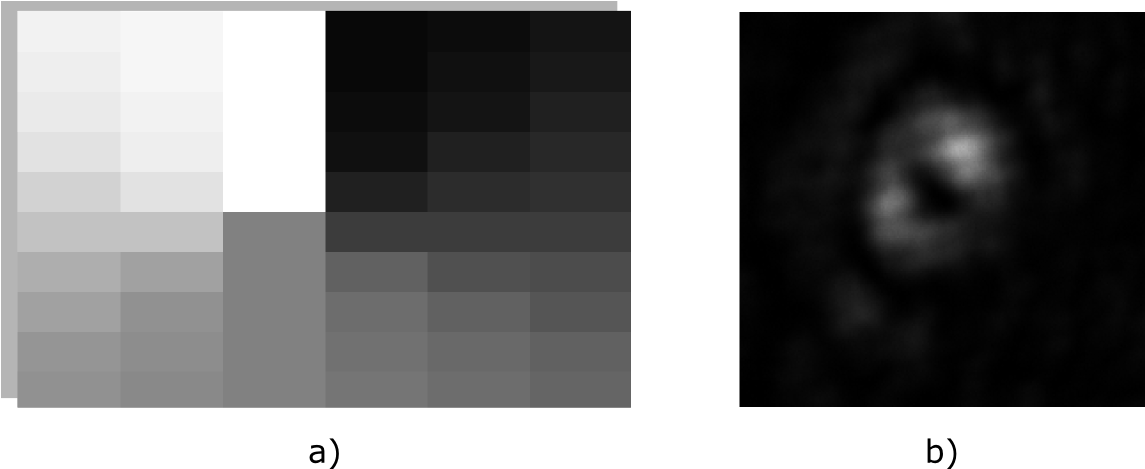
\includegraphics[ scale=.4]{discrete_mask.png}
%Las imagenes que enviamos al SLM son generadas en un
%  ordenador que de por sí es discreto, y llegan a un dispositivo
 % físico que tiene divisiones discretas, tanto espaciales como
 % electrónicas. Aún 
\caption[Efecto de pixelado en el SLM sobre las aberraciones en
VOs]{a) Magnificación de una mascara de fase espiral típica proyectada
  al SLM. b) Imagen de un VO de poca calidad producido con un SLM de 
transmisión modelo Holoeye LC2002.}
\label{fig:discrete_mask}
\end{figure}

Por otra parte, el SLM es discreto en la medida que sólo puede asignar
níveles de voltaje discretos (0-255 divisiónes de 5V) a cada una de
las celdas. Este fenómeno también es observable en la
Fig.~\ref{fig:discrete_mask}a) y puede introducir efectos 
indeseados. Más aún, si el modulador no llega a una
modulación de sólo fase, o si tiene una modulación que no llega al
rango de $2\pi$ radianes.  
Todas las posibles fuentes de error mencionadas anteriormente se
combinan para generar haces Laguerre-Gauss de poca calidad como el que se muestra
en la Fig.~\ref{fig:discrete_mask} b). 

Así tengan orígenes distintos, las fuentes de distorsión en
la fase del frente de onda pueden ser identificadas y corregidas como
una sóla aberración usando métodos de reconstrucción de fase. A
continuación presentamos un novedoso método de reconstrucción de fase
no interferométrico por medio del cual logramos identificar las
aberraciones de nuestro montaje óptico y corregirlas para generar VOs
de calidad.   

\subsection{Las técnicas de reconstrucción de fase no interferométricas}
\label{sec:ChPD_estado_del_arte}
\lhead{Caracterización de aberraciones en Vórtices Ópticos: \textit{Introducción}}
La presencia de aberraciones extrínsecas
%del último tipo 
en imágenes adquiridas por telescopios terrestres, y
la dificultad de modificar estos sistemas para incluir brazos de
referencia han sido las motivaciones principales para 
el desarrollo de varias \textbf{técnicas de Sensado de Fase no
Interferométricas} (\acrshort{NI-WFS}). La técnica de Diversidad de Fases o \textbf{Phase
Diversity} (\acrshort{PD}) pertenece a una familia de NI-WFS conocida como de
Reconstrucción de Fase o phase retrieval. A diferencia de técnicas
directas que requieren de óptica y sensores adicionales como los
sistemas que usan sensores Shack-Hartman, las implementaciones del PD
consisten en rutinas iterativas por medio de las cuales se 
logra determinar la fase de una función
compleja a partir de medidas de su magnitud usando 
información a priori de la función o de su transformada
\citepChPD{Fienup1993}. 
Una posible clasificación de las implementaciones del PD, se
da en la forma en la cual se lleva a cabo el proceso iterativo. Por un
parte, están los algorítmos en los cuales la fase se encuentra luego de
simular múltiples propagaciones, y por el otro las aplicaciones en las
cuales se encuentra la fase por medio de algorítmos de minimización
basados en la búsqueda del gradiente o \textbf{Gradient Search
  Algorithms} (\acrshort{GSAs}) \citepChPD{Fienup1982}. 
En términos generales, el tipo de implementación a usar depende de la
fuente a analizar; las aberraciones presentes en sistemas que hacen
imagen de fuentes distantes (como las estrellas) son caracterizadas
con implementaciones de PD que se basan en múltiples propagaciones
siguiendo esquemas como el método de \textbf{Gerchberg-Saxton} (\acrshort{GS})
\citepChPD{RWGerchberga}. Por otra parte, las implementaciones basadas en GSAs son
usadas para mejorar la resolución de sistemas que hacen imagen de
fuentes incoherentes y dispersas como por ejemplo la superficie del
sol \citepChPD{Bonet2005}.  
% Esta determinación puede consistir en un
% proceso de múltiples propagaciones cómo es el caso o en 
La técnica de PD ha sido usada
exitosamente en el contexto de sistemas de AO para incrementar la
resolución de sistemas ópticos 
tales como el Telescopio Espacial Hubble \citepChPD{Fienup1993}, y en
post procesamiento de imágenes de astronomía en las cuales la
resolución es crítica. Dos casos muy relevantes son el estudio de
manchas solares y la detección de planetas extrasolares \citepChPD{Lofdahl1994,Korkiakoski2012,Sauvage2007,Sauvage2012}. 
Así como con otras técnicas desarrolladas para aplicaciones en
astronomía, los métodos de reconstrucción de fase como el
GS y el PD han migrado a aplicaciones en el
laboratorio, y más específicamente a aplicaciones en microscopía de
fase \citepChPD{Jesacher2007,Camacho2010,Kner2013}. Tal es el caso
del trabajo de \citetChPD{Jesacher2007} que implementó una versión del
método GS mejorada con VOs para la optimización de sistemas de
generación de pinzas ópticas en un montaje de microscopía de
contraste de fase espiral.  Ellos mostraron que el uso de VOs a la
entrada del sistema óptico era más adecuado que los haces con fase
plana para la caracterización de aberraciones porque las
singuladridades ópticas que portan tinen mayor sensibilidad a la 
presencia de aberraciones. 

En este capítulo se presenta un método novedoso de reconstrucción de
fase del tipo PD, que se encuentra en el proceso de publicación en la
revista Optics Letters. Éste método fue desarrollado por el Grupo de Óptica Aplicada en
colaboración con un investigador de la Universidad de Medicina de
Harvard y es una variación del PD tradicional basada en GSAs, en la
cual se asume iluminación coherente a la entrada. Como en el método de
\citetChPD{Jesacher2007}, éste también es mejorado con VOs y la
introducción de una nuevo funcional permite determinar con gran exactitud las
aberraciones de sistemas ópticos formadores de imagen como es el caso
de sistemas 4F.  Específicamente, con este método logramos corregir las aberraciones ópticas
de un sistema formador de imagen en el cual se introducen las
diversidades con el SLM ubicado en un plano de Fourier.
Lá técnica que propusimos consiste en tomar imágenes con multiples
diversidades de fase introducidas por el SLM, y minimizar un funcional 
para obtener las aberraciones del sistema óptico. 
Creemos que una vez caracterizado, un sistema óptico formador de
imagen simple como el que presentamos, puede ser usado como una herramienta para
caracterizar aberraciones en sistemas formadores de imagen generales;
ya que al ser ubicado a la entrada de estos permite introducir
máscaras de diversidad de fase con efectos conocidos con las cuales se
puede ejecutar de nuevo el proceso de caracterización sobre el sistema
combinado. Se espera que por medio de un convenio de colaboración con
el Instituto Nacional de Técnica Aeroespacial de España  (INTA) se
pueda probar esta conjetura en sistemas ópticos
complejos para uso en astrofísica. 

A continuación, se presenta el marco teórico que
soporta la implementación del método. En la sección
\ref{sec:ChPD_materiales_y_metodos} se presenta el montaje óptico y se
describe el algoritmo general para la reconstrucción de fase. Luego, en
la sección \ref{sec:ChPD_resultados} se presentan los resultados de
simulaciones y experimentos que permiten corroborar la efectividad del
método para la corrección de aberraciones. 

\section{Marco Teórico}
\label{sec:ChPD_marco_teorico}
\lhead{Caracterización de aberraciones en Vórtices Ópticos:
  \textit{Marco Teórico}}
Los métodos de reconstrucción de fase no interferométricos dependen de
la medida de la intensidad del campo óptico que se
propaga a traves de un sistema formador de imagen. Si el sistema
formador de imagen se
caracteriza por su \textbf{función de dispersión de punto} (\acrshort{PSF}), la intensidad
a la salida puede ser descrita como una convolución entre la imagen a
la entrada y la PSF tal y como se ilustra en la Eq.~(\ref{eq:Output_Image}).
\begin{equation}\label{eq:Output_Image}
d(\vec{x}) = d_{obj}(\vec{x}) \otimes s(\vec{x}).
\end{equation}
En este caso hemos usado la notación de \citetChPD{Paxman1992} dónde
la PSF se representa como $s$, $d_{obj}$ es la intensidad del objeto a
la entrada y $d$ es la intensidad de la imagen a la salida, todas
ellas evaluadas en el espacio de coordenadas naturales ($\vec{x}$). El
 \href{http://es.wikipedia.org/wiki/Teorema_de_convolución}{teorema de
   convolución} permite representar la operación de la Eq.~(\ref{eq:Output_Image}) como un simple producto punto entre las
 \textbf{Transformadas de Fourier} (\acrshort{FT}s) de la intensidad a la entrada y la
 PSF como se muestra a continuación. 
\begin{equation}\label{eq:Output_Image_fourier}
D(\vec{u}) = D_{obj}(\vec{u})S(\vec{u}).
\end{equation}
En la Eq.~\ref{eq:Output_Image_fourier} el término $S$ denota la \textbf{Función de
Transferencia Óptica} (\acrshort{OTF}) del sistema formador de imagen, y así como
con los otros términos, letras mayúscula denotan una transformada de
Fourier sobre la función con notación minúscula.
\begin{align*} 
S(\vec{u})&= \mathcal{F}\{ s(\vec{x}) \},&D(\vec{u})&= \mathcal{F}\{ d(\vec{x}) \}, &D_{obj}(\vec{u})&= \mathcal{F}\{ d_{obj}(\vec{x}) \}. 
\end{align*}
Hasta el momento hemos trabajado únicamente con funciones reales que
representan la intensidad del campo punto a punto en los planos objeto
e imagen de un sistema óptico. Este tipo de notación es de gran utilidad para las
aplicaciones clásicas del método PD que hacen imagen de objetos
extendidos, y con fuentes de iluminación no coherentes. Sin embargo, en
sistemas ópticos con fuentes de iluminación coherentes, como el que se
presentó en la primera parte de este documento 
para la generación de VO, tenemos la ventaja de trabajar con
campos complejos que proporcionan información de amplitud y fase. Para
adaptar el método clásico de PD a una versión de iluminación coherente
es necesario trabajar con campos complejos. Es bien sabido que la OTF
y la PSF forman un par de Fourier en el dominio no coherente, y cada
una de ellas tiene un equivalente en el dominio de la luz
coherente. De un lado, la contraparte coherente de la PSF es la
Función de Respuesta al Impulso en amplitud o PSF de amplitud y de
aquí en adelante se denotará como $h(\vec{x})$. La PSF es el módulo
cuadrado de la \textbf{PSF de amplitud} (\acrshort{APSF}), 
\begin{equation}\label{eq:PSF}
s(\vec{x}) = |h(\vec{x})|^2.
\end{equation}
Y así como la PSF relaciona intensidades de campo a la entrada y salida de
un sistema por medio de una convolución, la APSF relaciona
los campos ópticos complejos,
 \begin{equation}\label{eq:Output_Image_complex}
u(\vec{x}) = u_{obj}(\vec{x}) \otimes h(\vec{x}).
\end{equation}
Por otra parte, el equivalente coherente de la OTF es la Función de
Transferencia Óptica de amplitud, o \textbf{Pupila Generalizada} (\acrshort{GP}) del sistema
y por ser el par de Fourier de la APSF se cumple la Eq.~(\ref{eq:GP}). 
\begin{equation}\label{eq:GP}
 H(\vec{u}) = \mathcal{F} \{h(\vec{x})\} =  A(\vec{u}) e^{i\phi(\vec{u})}
\end{equation}
En la Eq.~(\ref{eq:GP}) se observa que fuera de ser la FT de la APSF, la GP es
una función compleja que describe tanto la forma y
tramitancia de la apertura $A(\vec{u})$ como la fase introducida por sistema
óptico $\phi(\vec{u})$ en un plano de Fourier. La fase $\phi$ generalmente es sinónimo de las
aberraciones del sistema y se describe matemáticamente de forma
parametrizada como una combinación de polinomios de Zernike
\footnote{El anexo \ref{cha:Anexo3} hace referencia a los polinomios
  de Zernike y a la composición de aberraciones en esta base.}
\citepChPD{Paxman1992}. Finalmente, la OTF de un sistema formador de
imagen con iluminación coherente se puede obtener mediante la
autocorrelación normalizada de la GP como se muestra a continuación,
\begin{equation}\label{eq:OTF}
S(\vec{u}) = \frac{H(\vec{u}) \star H(\vec{u})}{|H(\vec{u})|^2}.
\end{equation}
Todo lo mencionado anteriormente ha sido ingeniosamente condensado por
\citetChPD{UribePatarroyo2011} en una versión de la Fig.~\ref{fig:ChPD_kernels_sistemas_formadores_de_imagen}. 
\begin{figure}[h!]
\centering
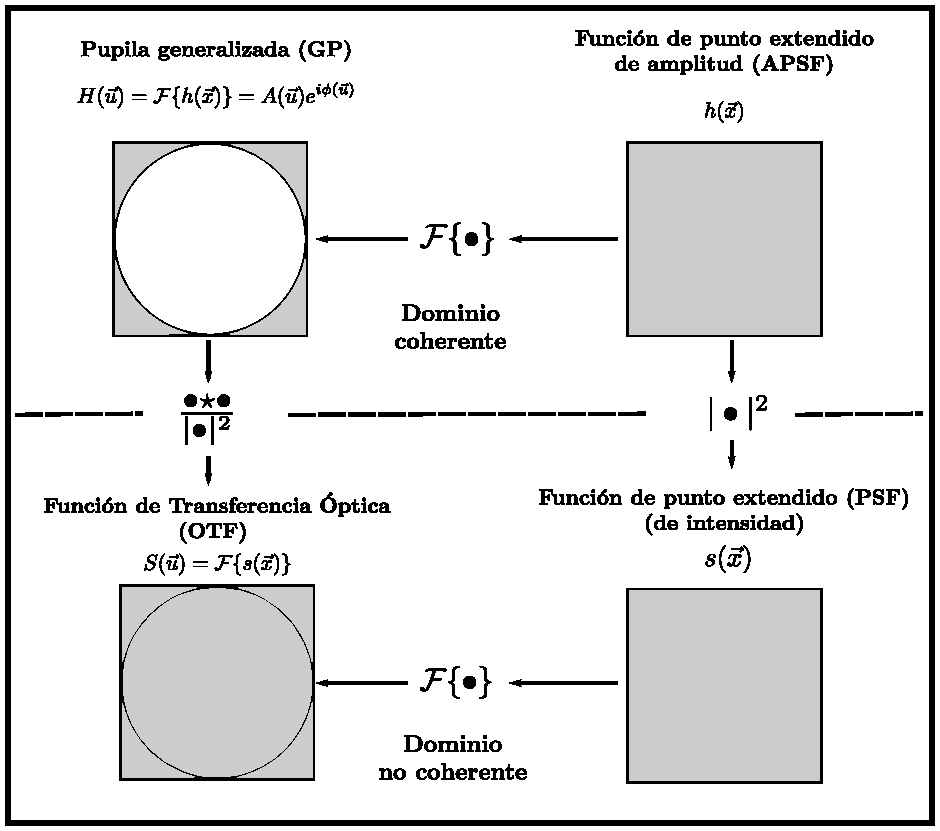
\includegraphics[scale=.8]{kernels_sistemas_formadores_de_imagen.pdf}
\caption[Relaciones entre funciones de transferencia ópticas y sus FT.]{Relaciones entre funciones de transferencia ópticas y sus
  transformadas de Fourier en los dominios coherente y no
  coherente. Inspirado en una versión similar de \citetChPD{UribePatarroyo2011}.}
\label{fig:ChPD_kernels_sistemas_formadores_de_imagen}
\end{figure} 
Ahora bien, las expresiones (\ref{eq:PSF}) y (\ref{eq:OTF}) nos
permiten llevar sistemas ópticos descritos por campos complejos a la
notación tradicional del PD. A continuación se describen los aspectos
 generales de la reconstrucción de fase con PD, en la sección
 \ref{sec:ChPD_PD_il_coherente} se describirán las modificaciones que
 hacemos al PD tradicional para aprovechar el tipo de iluminación no
 coherente, y en la sección \ref{sec:ChPD_PD_Spiral_Diversity} se
 explica el efecto de introducir máscaras espiral como diversidades de
 fase. 

\subsection{Phase Diversity tradicional}
\label{sec:ChPD_PD_tradicional}
Si la GP del sistema es modificada por un cambio conocido en la fase o
diversidad de fase de la forma,
$$H_{\Delta}=e^{\phi_1(\vec{u})},$$ 
obtenemos una nueva GP que se puede describir como el producto entre
la GP original ($H_{0}$) y la GP con el cambio o diversidad de fase
($H_{\Delta}$). Estas diversidades son generalmente desenfoques
introducidos al cambiar el camino óptico de haces esféricos, o pueden
ser otro tipo de distribuciones de fase fácilmente parametrizables en
polinomios de Zernike como el astigmatismo. Tomando la autocorrelación normalizada de la GP con
diversidad como se muestra en la Eq.~(\ref{eq:first_diversity_OTF}),
\begin{equation}\label{eq:first_diversity_OTF}
S_1 = \frac{H_1\star H_1}{|H_1|^2} = \frac{H_0H_{\Delta} \star H_0H_{\Delta}}{|H_0H_{\Delta}|^2},
\end{equation}
obtenemos una OTF con diversidad $\phi_1$ que nos permitirá predecir cómo son
las imagenes registradas a la salida del sistema cuando se introduce
un cambio de fase, $$D_1 = D_{obj} S_1.$$ 
La tarea de encontrar las aberraciones del sistema óptico en el PD
tradicional consiste entonces en encontrar una distribución de fase
inicial $\phi(\vec{u})$ que en combinación con la función pupila
$A(\vec{u})$ componga una OTF capaz de modelar el
sistema. Esta OTF debe predecir, a partir de una entrada dada 
($D_{obj}$)  no solo la imagen nominal ($D_0$), sino tambien
las imágenes distorsionadas $D_{1...k}$ que resultan de la adición de
$k$ diversidades de fase distintas. Y la adición de más de una
diversidad de fase es lo que diferencia al método PD de métodos
similares, en particular, la inclusión de diversidades implica que la
fase del frente de onda recuperado debe ser una solución para un
conjunto de sistemas y no sólo para uno, esto le otorga al método una
mayor exactitud. Las implementaciones de PD basadas en GSAs, como por
ejemplo la de \citetChPD{Paxman1992}, usan
métodos de búsqueda de la mayor pendiente para 
minimizar funcionales de la forma,
\begin{equation}\label{eq:metric}
L(\bar{D}_{obj}, \phi)= \sum_{j=0}^{K} \sum_{u,v}^{M,N}  \left |D_{j} - \bar{D}_{obj} S_{j} \right | ^2.
\end{equation}

Dónde $\bar{D}_{obj}$ es la FT del objeto a la entrada limitada por las frecuencia
de corte establecidas en la apertura, y $D_{j}$ es la FT de la intensidad
medida experimentalmente por una cámara en el pixel con coordenadas $\vec{u}$ luego de
introducir una diversidad de fase conocida con índice $j$.      
Este funcional actua como una medida de la similitud entre la
intensidad de un objeto que se propaga por un sistema modelado por
$S_{j}$ y la medida real de su imagen. Obtener un valor mínimo al
evaluar el funcional para todas las diversidades $j$ implica que el objeto a la entrada y la OTF del
sistema se conocen de forma suficientemente precisa como para emular
el sistema real.   

Es importante fijarse en que el funcional clásico de PD de la
Eq.~(\ref{eq:metric}) debe solucionarse simultaneamente con respecto a
dos variables. Esto se debe a que en aplicaciones de PD para sensado
remoto se desconoce tanto la fase introducida por el sistema, como las
propiedades del objeto a la entrada \citepChPD{Bonet2005}. Puesto que solucionar un funcional
simultaneamente para dos funciones resulta complejo y muy costoso
computacionalmente, desde los inicios de la técnica autores como
\citetChPD{Gonsalves1982} han propuesto 
una transformación de la Eq.~(\ref{eq:metric}) que permite describir el funcional sólo en términos
de la fase del frente de onda. Esta transformación está descrita
de forma muy completa y generalizada en el trabajo de
\citetChPD{Paxman1992}.
% y ha sido implementada exitosamente por \citetChPD{Katkovnik2012}. 
No obstante, ha sido demostrado que la forma reducida del funcional es
mucho más susceptible a devolver mínimos locales en la presencia de
ruido Gaussiano, y por tanto, se ha propuesto el uso de métodos de
regularización y metaheurísticos para incrementar la convergencia \citetChPD{Paxman1992}.  

En la siguiente sección se propone traer los conceptos del PD
tradicional a sistemas que pueden ser iluminados con fuentes
coherentes como aquellos donde son aplicables métodos de
propagaciones iterativas como el método de GS.

% una modificación al PD clásico que
% soluciona estos problemas con la condición de limitar el método a
% rangos de aplicación en los cuales es posible conocer el frente de
% onda a la entrada del sistema óptico. 

\subsection{PD con iluminación coherente}
\label{sec:ChPD_PD_il_coherente}

La variación de PD que nosotros proponemos puede llamarse PD con
iluminación coherente, e implica asumir un frente de onda a la entrada
del sistema. 
Como se mencionó antes, el sistema óptico a caracterizar es un sistema
4F compuesto por dos lentes. La razón por la que se escogío este tipo
de sistemas formadores de imágen es porque a futuro se espera utilizar
los VOs generados para aplicaciones en microscopia de fase dónde
ubicar un SLM en un plano de Fourier puede permitir la introducción de
filtros y máscaras que mejoren el contraste de muestras biológicas transparentes
\citepChPD{Maurer2011}. 
Dado que usamos  una fuente láser para generar VOs, podemos asumir que el campo óptico a la entrada, $u_{obj}$, se puede representar
como un haz de luz coherente con perfil Gaussiano,
$$u_{obj} = e^{\frac{-(x^2+y^2)}{\sigma}}.$$
 Ese sería el campo óptico en el plano objeto, es decir, a una
 distancia focal de la primera lente. La FT del 
 objeto , $U_{obj}$ puede ser
 observada en el plano focal de la
 primera lente (2F), que es también el plano de Fourier del
 sistema. Es allí donde se ubica el SLM para proyectar máscaras de
 fase con diversidades. Luego, el campo a la salida del sistema, que
 ha sido modificado por las distintas aperturas y aberraciones del sistema se puede
 observar en el plano imágen a 4 distancias 
 focales del plano objeto. Si se define la GP como el producto entre
 la GP asociada a las aberraciones del sistema ($H_0$) y a las diversidades
 introducidas por el SLM ($H_j$), usando la Eq.~\ref{eq:Output_Image_complex} el
 campo a la salida se puede expresar en términos del campo a la
 entrada como se muestra en la Eq.~\ref{eq:field}.
\begin{equation}\label{eq:field}
u_{j}(\vec{x}) = \mathcal{F}^{- 1}\{ U_{obj} H_0(\vec{u}) H_j(\vec{u}) \}.
\end{equation} 
Con la Eq.~(\ref{eq:field}) se puede plantear un equivalente coherente del
funcional de la Eq.~ (\ref{eq:metric}) en el cual la única incógnita son las
aberraciones ($\phi$) introducidas por el sistema óptico,
\begin{equation}
L_j(\phi)= \sum_{j=0}^{K} \sum_{u,v}^{M,N}  \left |d_{j} - |u_j|^2
\right | ^2.
\label{eq:metric_coherent}
\end{equation}
Si la apertura es circular y el objeto es un haz Gaussiano, las
distribuciones de intensidad a la salida para cada diversidad
($d_{j}$) son patrones de Airy distorsionados, y localizados en el centro de la imagen.  
Es importante notar que a diferencia del PD tradicional, nosotros
comparamos las imágenes en coordenadas naturales en vez del dominio de
frecuencia espacial. Esto se debe a que analizamos las distribuciones
de intensidad que
produce un sistema formador de
imágenes cuando se introducen las máscaras con diversidades en un
plano de Fourier. Otra diferencia muy importante es que podemos saber
cómo será la fase a la salida, cosa que no se podría hacer con
iluminación no coherente. Esto es esencial si queremos garantizar un
perfil de fase específico como por ejemplo una vorticidad particular. 

\subsection{Máscaras espirales como diversidades de fase}
\label{sec:ChPD_PD_Spiral_Diversity}
Como se mencionó en la introducción, \citetChPD{ Jesacher2007}
propusieron el uso de máscaras espirales para mejorar el desempeño en
la reconstrucción de aberraciones por medio del método GS en un
sistema formador de imagen. El GS es un método iterativo de
reconstrucción de fase que funciona con sólo una imagen como
entrada. En ese trabajo mostraron que si el sistema
óptico se ilumina con haces portadores de OAM 1, la imagen a la salida
(que tiene forma de dona) responde con mucha mayor sensibilidad a aberraciones que las
imagenes observadas cuando la iluminación es de fase plana (OAM 0). Ese
incremento en la sensibilidad se ve traducido en una mayor
precisión, y en un aumento en la convergencia que hacen del método una alternativa
atractiva para la optimización de sistemas ópticos en los cuales se
necesita contról preciso de la fase. 

Nosotros también proponemos el uso de VOs para mejorar la exactitud de
la reconstrucción, pero llevamos la idea más adelante al proponer el
uso VOs no como una fuente de iluminación sino como una nueva familia
de diversidades que se combina con las diversidades usadas
tradicionalmente en el PD como el desenfoque y el astigmatismo. La
introducción de estas nuevas diversidades al método de PD con
iluminación coherente se logra si se modifica el funcional de la
Eq.~(\ref{eq:metric_coherent})  para recibir diversidades de fase que
introduzcan OAM al haz de entrada.
Estas diversidades son máscaras espiral de fase parametrizadas por el
valor de su carga topológica $l$ y definidas como:
$$\psi_l = arg(\exp{(il \theta)}),$$
tál y como se mostró en el capítulo \ref{sec:OV_gen}. 

Al incluir las máscaras espiral en un plano de Fourier del sistema, la fase del frente de
onda se puede representar aproximadamente como la suma de:
\begin{itemize}
\item Las aberraciones inherentes al sistema ($\phi$) representadas como una
  combinación ponderada de polinomios de Zernike. En nuestro caso la
  combinación se hace con los primeros 15 coeficientes siguiendo la
  convención de numeración de \citetChPD{Noll1976}. 
\item La diversidad de fase espiral $\psi_l$.
\item La diversidad de fase de aberración $\phi_j$ que consiste en
  un solo elemento de la base de Zernike, como desenfoque o
  astigmatismo. 
\end{itemize}
El campo complejo a la salida del sistema cuando se introduce una diversidad de
aberración $j$ y una diversidad de espiral de fase $l$ en un plano de
Fourier es entonces,
\begin{equation}\label{eq:newGP}
 u_j^l =  \mathcal{F}^{- 1}\{U_{obj} A e^{i\left(
     \phi+ \psi_l + \phi_j \right)} \}.
\end{equation}

Finalmente, usando la Eq.~(\ref{eq:newGP}) se puede definir el funcional de
PD coherente mejorado con VOs que se muestra en la Eq.~(\ref{eq:metric_coherent_OAMs}). %a continuación:
\begin{equation}\label{eq:metric_coherent_OAMs}
L(\phi)= \sum_{l=0}^L\sum_{j=0}^{K} \sum_{u,v}^{M,N}  \left |d_{j}^l - |u_j^l|^2 \right | ^2.
\end{equation}
Con este funcional se puede plantear una metodología de solución para
el problema de reconstrucción de fase como se ilustra en el diagrama
de flujo de la Fig.~\ref{fig:flowchart}.
\begin{figure}[h!]
\centering
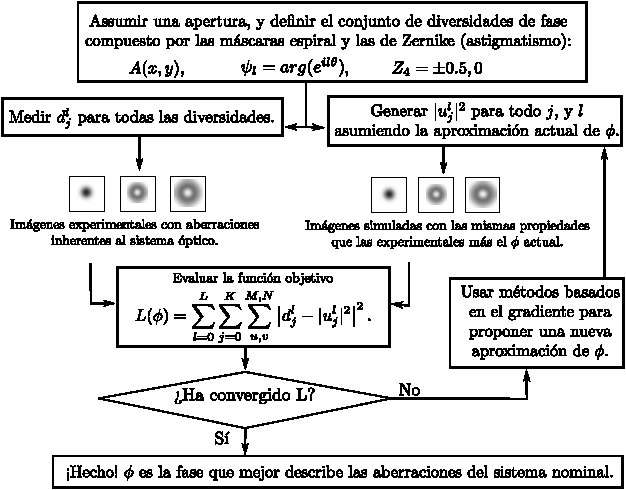
\includegraphics[scale=1.2]{PDLightFlux_simple_esp.pdf}
\caption[Diagrama de flujo del PD con iluminación coherente]{Diagrama de flujo de una implementación de PD con iluminación
  coherente mejorado con VOs.}
\label{fig:flowchart}
\end{figure}
A continuación, en lo que resta de este capitulo se ahondará en los
detalles de la metodología, y se presentarán los 
resultados obtenidos.

\section{Metodología}
\label{sec:ChPD_materiales_y_metodos}
\lhead{Caracterización de aberraciones en Vórtices Ópticos:
  \textit{Metodología}}
Como se mencionó en la Sección \ref{sec:ChPD_PD_il_coherente}, para
poder generar imágenes simuladas $|u_j^l|^2$ nuestro método se basa en
la premisa de conocer el campo óptico a la entrada del sistema
formador de imagen. Es decir que si usamos un láser de buena calidad
para obtener las imágenes del brazo izquierdo del diagrama en la Fig.~\ref{fig:flowchart} podemos asumir que el campo a la entrada del
sistema simulado ($u_{obj}$) 
%que produce las imágenes del brazo derecho
, tiene las características
ópticas de una fuente láser coherente, es decir: amplitud Gaussiana, perfil
de fase plano, y que además está limitado por una
apertura circular correspondiente a la geometría de las lentes.  

Como el nuestro es un sistema formador de imagen y vamos a introducir las
máscaras de diversidades en un plano de Fourier para simular la
autocorrelación, se debe obtener la transformada de Fourier del campo
mencionado anteriormente y colimar el haz para evitar que siga
divergiendo. En adelante haremos 
referencia a la Fig.~\ref{fig:set-up} para ilustrar las diferentes
partes del sistema de reconstrucción de fase como si se tratara de
un sistema 4F.
Suponiendo que el frente de onda ya ha sido transformado al dominio de Fourier y que se
encuentra colimado, representamos en el extremo izquierdo de la Fig.~\ref{fig:set-up} la FT del campo a la entrada ($U_{obj}$) como un haz
circular que incide sobre el SLM.  Dado que el campo ha sido
colimado luego de obtener su FT, se puede asumir que todos los planos desde que
se colima el haz hasta que vuelve a pasar por una lente son
equivalentes al plano de Fourier de un sistema 4F, y eso nos brinda un
espacio adecuado para introducir el SLM como se muestra en el recuadro
azul de la Fig.~\ref{fig:set-up}. 

Si se trabaja en aplicaciones de microscopía, en las cuales los objetos
son de tamaños micrométricos, sus transformadas de Fourier son campos
ópticos más extensos y la información en coordenadas de frecuencia
espacial puede dispersarse en tamaños comparativamente más
grandes. Una ventaja significativa de modificar el PD para que las
diversidades de fase se introduzcan en un plano de Fourier es el hecho
de que se pueden aprovechar más pixeles, y por ende se aumenta la
resolución espacial de la modulación de fase. 

%El uso de SLMS y sus ventajas. 

El uso de dispositivos de modulación espacial de la fase para
aplicaciones en PD se ha extendido en la literatura
\citepChPD{Uribe-Patarroyo2010,Camacho2010,Korkiakoski2012,Katkovnik2012}
debido a la flexibilidad con la que se pueden generar máscaras de fase
arbitrarias como diversidades de fase, a diferencia de métodos
tradicionales como desenfoques que dependen de desplazamientos y alineación muy
precisos de elementos ópticos. Más aún, el uso de elementos de
la base de Zernike (diferentes al desenfoque) como diversidad de aberración tiene la ventaja de
producir distorsiones más grandes y más facilmente detectables en la
distribución de intensidad del plano imagen. Esto es particularmente
cierto cuando las distribuciones pertenecen a objetos altamente
sensibles a aberraciones como es el caso de los OVs. Adicionalmente, polinomios de
Zernike como los dos correspondientes al astigmatismo primario han
sido usados por \citetChPD{Kner2013} como diversidad de aberración en
PD para reconstrucción de fase de objetos tridimensionales en
aplicaciones de microscopía donde el desenfoque es usado para
muestrear en la dirección del propagación y no añade información
sobre las aberraciones.  
 
\begin{figure}[h!]
\centering
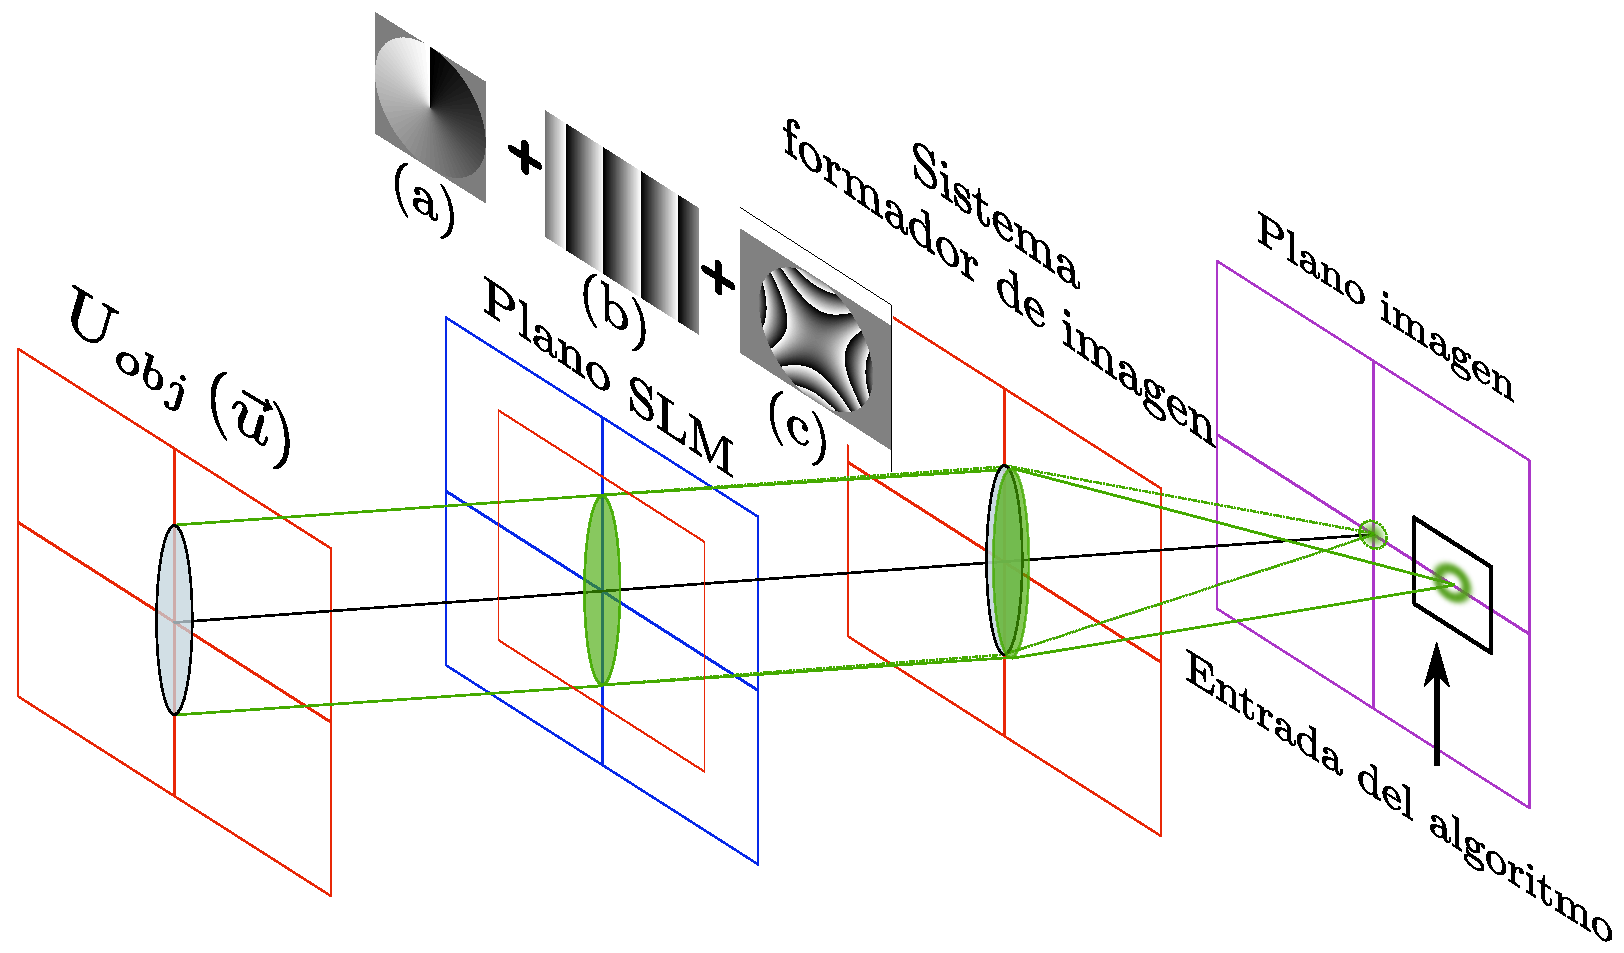
\includegraphics[scale=.5]{PhaseDiversitySetup_esp.pdf}
\caption[Diagrama del sistema óptico para PD con iluminación coherente.]{Un SLM es usado para introducir diversidades de fase en un
  plano de Fourier. La máscara que se asigna al SLM es una combinación de:
  (a) Máscara espiral de fase con OAM 1, (b) rejilla de difracción
  tipo Blazed, y (c) +0.5 astigmatismo primario como diversidad de
  aberración. El primer orden de difracción producido por la rejilla
  es usado como portador de los haces Laguerre-Gauss con OAM1
  enfocados en el plano imagen.} 
\label{fig:set-up}
\end{figure}

Cuando el campo $U_{obj}$ llega al SLM se encuentra con una combinación de tres
máscaras de fase que han sido asignadas a los píxeles del LCD. La
primera de estas máscaras, visible en la Fig.~\ref{fig:set-up}(a)  es una máscara de espiral de fase con carga
topologica $l$ que, como se vio en el Capítulo \ref{sec:OV_gen}, introduce un una
singularidad de fase de orden $l$ al campo. La segunda máscara
(Fig.~\ref{fig:set-up}(b)) corresponde a una rejilla de difracción del tipo
blazed que representa una cuña delgada, y se usa para separar la luz
que ha sido difractada al primer orden del resto. 
Esta rejilla mejora de forma significativa la calidad
de los vórtices ópticos porque evita efectos de interferencia causados
por partes del campo que no son correctamente difractadas por el
modulador. La poca eficiencia de difracción se debe a la no linealidad
de la modulación y al hecho de que los TN-SLM de transmisión no logran
modulaciones de $2\pi$.  Finalmente, la tercera máscara
(Fig.~\ref{fig:set-up}(c)) introduce la diversidad de fase de
aberración, en este caso, y en adelante,  corresponde al polinomio de
Zernike de astigmatismo primario (De índice 4 en la notación de
Noll). La suma de las tres máscaras tal y como se le presenta al SLM
en el montaje experimental se muestra en la Fig.~\ref{fig:mixed_mask} superpuesta a una
apertura circular que corresponde al tamaño del haz en el SLM.   

\begin{figure}[h!]
\centering
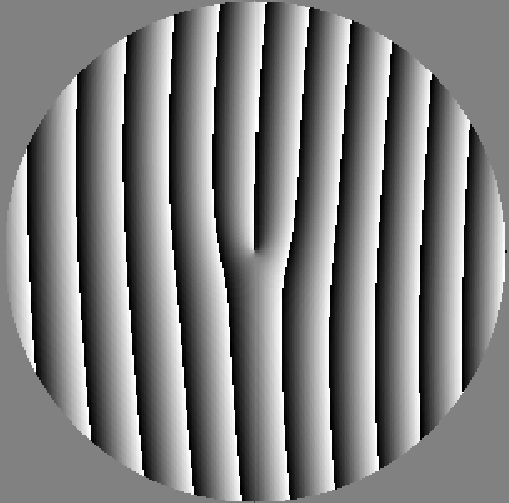
\includegraphics[scale=.5]{mixed_mask_compact.pdf}
\caption[Ejemplo de una máscara tenedor con astigmatismo.]{Ejemplo de una máscara tenedor que resulta de combinar una
  máscara de espiral con $l=1$, con una red de difracción y una
  máscara de diversidad de aberración con astigmatismo primario de
  $Z_4=0.5\lambda$. Se muestra sólo la parte de la imagen que tiene el
tamaño del haz proyectado en el SLM.º} 
\label{fig:mixed_mask}
\end{figure}

Luego de atravesar el SLM el haz encuentra el resto del sistema óptico
y se enfoca para formar imagen ($|u_j^l|^2$) en el plano de observación o plano
imagen. 
% En nuestro caso el resto del sistema consiste en una sola
% lente (tal y como se muestra en alguna foto) con la misma curvatura
% que la lente usada para colimar el haz hace ima. 
Como se puede ver en el extremo derecho de la figura \ref{fig:set-up},
los perfiles de intensidad que se usan como entrada para el algoritmo
de la figura \ref{fig:flowchart} corresponden sólo a una pequeña parte
de la imagen en la cual está el orden +1 de la rejilla de
difracción. Dado que los spots tienen un tamaño microscópico, para observar sólo
el orden 1 en el plano de enfoque usamos un objetivo de 
microscopio de magnificación 10x y una cámara \acrshort{CCD} marca Imaging
Source.    

% \begin{mdframed}[hidealllines=true,backgroundcolor=blue!20]
\emph{En conclusión, para realizar la reconstrucción de fase de un sistema
óptico formador de imagen usando nuestro método, se deben registrar varias de las
imágenes que éste forma cuando se le introducen cambios conocidos en
la fase. Los cambios en la fase se introducen a partir de máscaras de
fase localizadas en uno de sus planos de Fourier por medio de un
TN-SLM.  
Introducir las máscaras de fase genera distorsiones en la distribución
a la salida que además dependen de las aberraciones ópticas desconocidas del
sistema en cuestión. El hecho de generar varias combinaciones de
diversidades y registrar varias imagenes con distorsiones distintas,
lleva a limitar el espacio de soluciones posibles y acerca el método a
una solución única. Esta es la gran ventaja del PD sobre otros métodos
de reconstrucción de fase.}
% \end{mdframed}


Adicionalmente, el hecho de usar la familia
de diversidades de espiral, aumenta la sensibilidad del método ante
aberraciones ya que los haces portadores de OAM tienen cambios más
drásticos en sus distribuciones de intensidad cuando hay
aberraciones. Aumentar la sensibilidad tiene un efecto positivo sobre
la exactitud de la solución porque se encuentra de forma más precisa
el valor y tipo de aberraciones que producen una distribución particular. 

El conjunto de imágenes tomadas experimentalmente ($d_j^l$), y las
condiciones particulares con las cuales fueron producidas, tales como:
la forma de la apertura, el tipo de iluminación y la selección de diversidades, son el
argumento de la rutina de PD. En el interior de la rutina de PD,
simulamos el sistema óptico y producimos imágenes artificiales
($|u_j^l|^2$) que son comparadas píxel a píxel con las imágenes
experimentales. Así como las distorsiones en las imágenes
experimentales son función de las aberraciones que desconocemos, las
distorsiones de las imágenes artificiales van a ser función de una
fase conocida y parametrizada ($\phi$) que vamos a variar hasta que el
funcional de la Eq.~\ref{eq:metric_coherent_OAMs} retorne un mínimo. 
Cuando acabe el esquema de búsqueda de un mínimo, y la fase
propuesta ($\phi$) produzca imágenes artificiales ($|u_j^l|^2$)
idénticas a las imágenes experimentales, y siempre y cuando las
condiciones de la simulación sean idénticas a las condiciones del
laboratorio, significará que hemos identificado las aberraciones del
sistema óptico correctamente. Adicionalmente, el inverso de las aberraciones
encontradas puede ser proyectado en el SLM para corregirlas y así mejorar la resolución
del sistema.

Una vez presentado el método, procedemos a describir los resultados
logrados. 
%introducir un TN-SLM en un plano de Fourier 

\section{Resultados}
\label{sec:ChPD_resultados}
\lhead{Caracterización de aberraciones en Vórtices Ópticos:
  \textit{Resultados}}
El método de PD coherente mejorado con VOs fue probado extensivamente
con el fin de validar nuestras premisas y evaluar su comportamiento ante diversas entradas. 
En esta sección se describen las pruebas simuladas y experimentales
que se realizaron, y se muestran los resultados para cada una. 

\subsection{Resultados de simulaciones}
\label{sec:ChPD_resultados_simulados}
En primera medida se requería simular el método para corroborar que
funcionaba en sistemas ideales. La simulación de reconstrucción de
fases consiste en reemplazar el conjunto de imagenes de referencia $d_j^l$ por un
conjunto de imágenes artificiales que han sido afectadas por una
aberración conocida inherente al sistema
óptico simulado. La aberración conocida será nuestra fase de
referencia, es decir, la fase con la cual compararemos la exactitud de
la reconstrucción. 
Una vez comprobamos que nuestra implementación del PD reconstruía de
forma precisa aberraciones simples, procedimos a probarlo con
aberraciones generadas aleatoriamente, y luego con aberraciones aleatorias de
diferente magnitud. Asimismo, comparamos el desempeño del PD contra el
método GS con y sin VOs, y contra sí mismo con conjuntos diferentes de
diversidades con y sin VOs.  

\subsubsection{Preparación de las fases de referencia}

Si las aberraciones se conforman como una combinación lineal de
elementos de la base de Zernike como se muestra en la
Eq.~\ref{eq:ChPD_phase_Zernike}; un frente de onda aleatorio puede ser 
facilmente compuesto asignando valores aleatorios a los coeficientes $a_i$. 
\begin{equation}
\label{eq:ChPD_phase_Zernike}
\phi(\vec{u}) = \sum_{i=1}^{N=15}a_iZ_i(\vec{u}). 
\end{equation}
Para generar los coeficientes utilizamos la función \textbf{normrnd}
de Matlab$\circledR$ que produce una lista de números aleatorios pertenecientes
 a una distribución Gaussiana con media y desviación
estándar definidas por el usuario.  En nuestro caso se quería una
misma probabilidad para coeficientes positivos y negativos así que se asignó la media
como $0\lambda$. La desviación estándar se asignó como $0.5\lambda$ como valor
tentativo previo al escalamiento.\\
La exactitud de los métodos de reconstrucción de fase en algunos casos
está ligada a la magnitud de las aberraciones. Aberraciones de
magnitud muy pequeña pueden producir resultados similares a
aberraciones de igual magnitud pero distinta forma. Esto es un
problema si los métodos no son lo suficientemente sensibles como para
distinguirlas. Asimismo, aberraciones de magnitudes muy altas pueden
introducir distorsiones tan grandes en las imágenes de entrada que
impiden que los métodos converjan a un mínimo global, o incluso pueden
causar divergencia \citepChPD{Jesacher2007}. Con el fin de evaluar el desempeño de nuestro
PD ante magnitudes variables, generamos aberraciones aleatorias en diferentes
escalas. Se tomó como métrica de la escala el valor de la \textbf{media
cuadrática} (\acrshort{RMS}) \citepChPD{Schmidt2010} del frente de
onda, que para una base normalizada como la de Zernike es,
$$RMS =  \sqrt{\sum_{i=1}^{N=15}a_i^2 }.$$
Los coeficientes aleatorios que entrega la función \textbf{normrnd}
fueron escalados en una rutina de minimización hasta obtener una
combinación con RMS definido.  
Se corrió la rutina de PD para 6 escalas distintas  $\sum_{i=1}^6\sigma_i$ desde
$RMS = 1/14\lambda$ (límite de 
difracción) hasta $RMS = 1\lambda$. Y cada una de las reconstrucciones
de una escala particular ($i$) fue repetida con fases distintas 15 veces
para que el resultado fuera estadísticamente significativo. Es decir
que en total se hicieron  90 reconstrucciones de fase por cada método
a evaluar. Se evaluó el método de GS con y sin VOs, y el método de PD
de iluminación coherente sin VOs, y con VOs bajo dos combinaciones
distintas de diversidades haciendo un total de 450 reconstrucciones de
fase.  
Los resultados de estas simulaciones se han condensado en la
Fig.~\ref{fig:ChPD_RMS_error} y se discuten en adelante.  
\begin{figure}[h!]
\centering
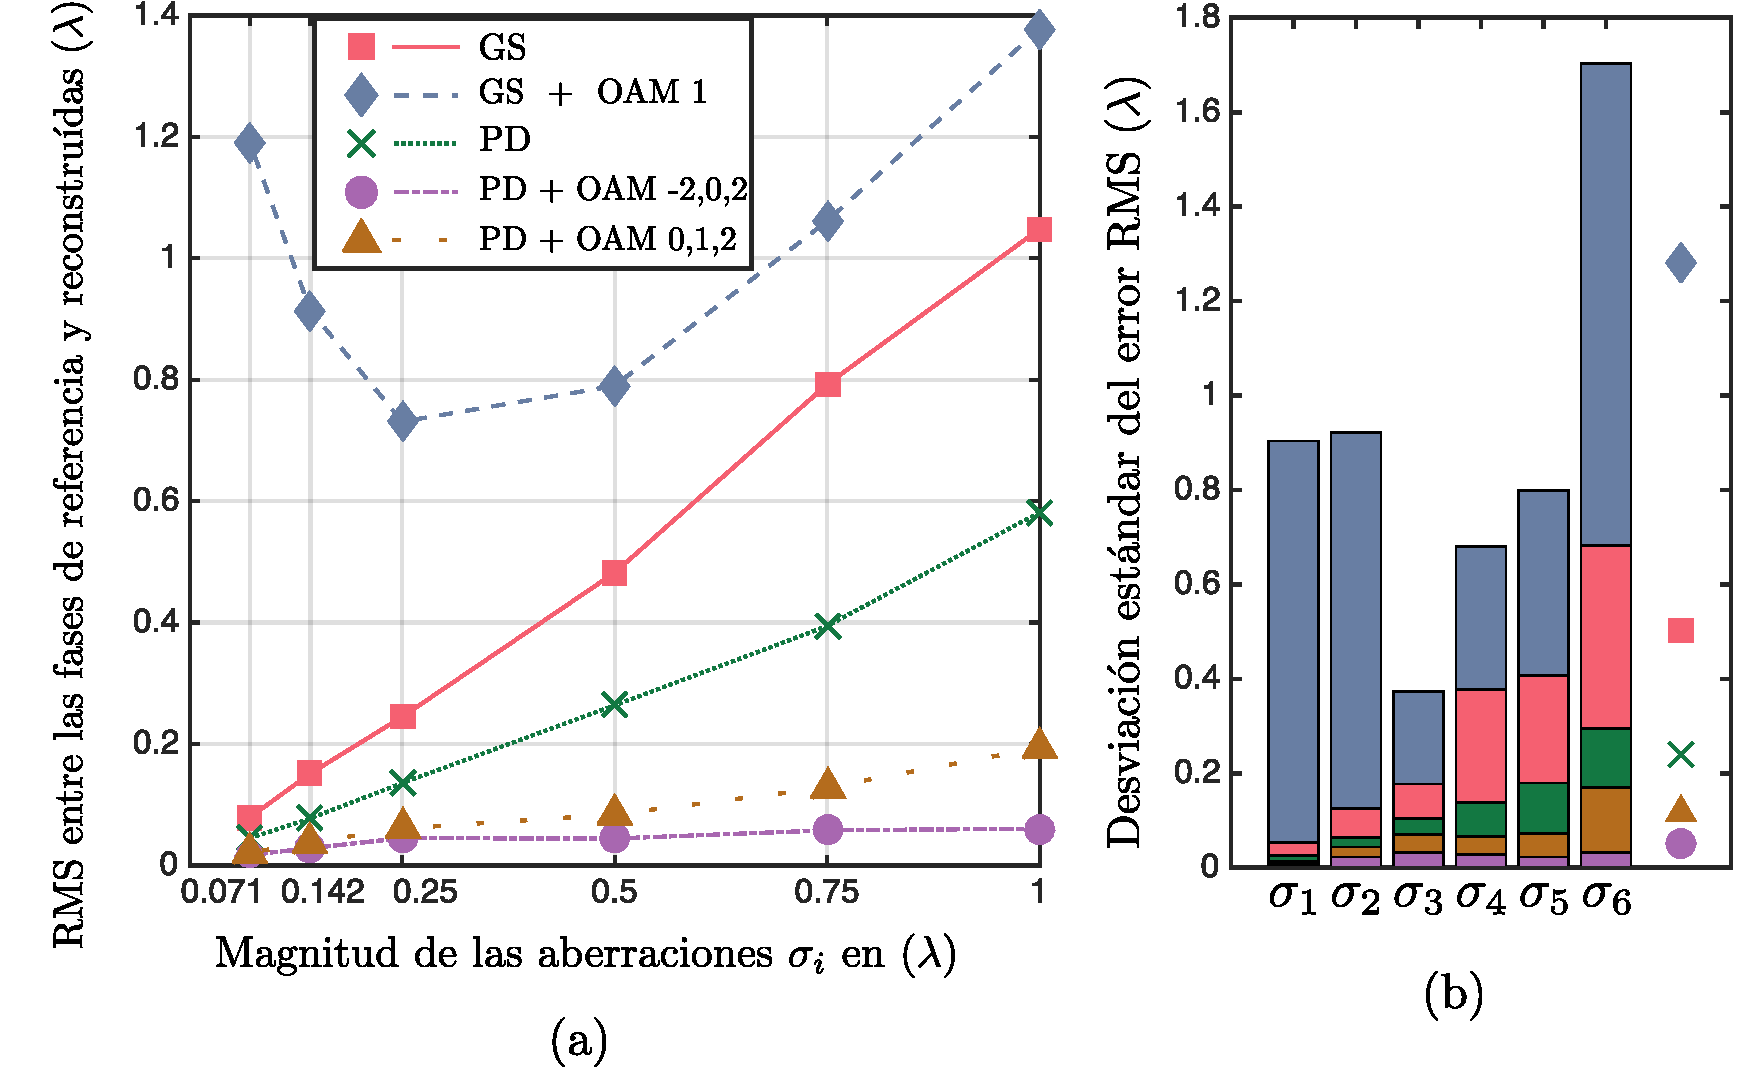
\includegraphics[scale=.5]{mixed_wf_errors_esp.pdf}
\caption[Resultados de simulaciones con PD de iluminación
coherente.]{(a) Las marcas en el eje $x$ denotan la magnitud de la
  aberración para cada escala $\sigma_i$ como el error RMS con
  respecto a un frente de onda plano. El eje $y$ denota el promedio de
  los errores RMS entre las 15 réplicas de aberración de referencia y
  fase reconstruída. (b) Desviación estándar del error para cada
  método y para cada $\sigma_i$.} 
\label{fig:ChPD_RMS_error}
\end{figure}

\subsubsection{Descripción y análisis de resultados simulados}
Comenzamos por describir brevemente los datos que componen las curvas
de la Fig.~\ref{fig:ChPD_RMS_error}(a). 
De un lado está la curva con marcas cuadradas rojas que representan el error 
para cada escala cuando se reconstruyen las aberraciones usando el
método GS tradicional. Los rombos azules son también resultado de la
reconstrucción con GS y
representan la solución cuando se añaden VO de OAM1 a la entrada, tal
y como lo presenta \citetChPD{Jesacher2007}. En ambos casos el GS se
ejecuto por 60 iteraciones. Por otra parte, del lado
de PD con iluminación coherente, los datos con cruces verdes
representan el método PD coherente cuando no ha sido mejorado con
diversidades de fase espiral.
%, presentado en la sección \ref{sec:ChPD_PD_il_coherente}. 
En ese caso se usaron sólo tres imágenes como entrada, la nominal y
dos con diversidades. No se usaron máscaras espiral ($l=0$), y las
diversidades de aberración consisten en los siguientes dos valores de
astigmatismo $j=Z_4:\pm 0.5$. Tanto los datos con triángulos dorados
como los que tienen círculos púrpura representan resultados del
método de PD con iluminación coherente mejorado con VO y fueron
obtenidos con nueve imágenes. Las diversidades de aberración para
estos casos son las mismas y se añaden las diversidades de espiral
$l=0,1,2$ para el primer caso y $l=-2,0,2$ para el segundo.  

En la Fig.~\ref{fig:ChPD_RMS_error} se puede observar claramente que
el método de PD coherente supera en 
exactitud al GS por al menos un orden de magnitud en cualquiera de las
selecciones de diversidades. La precision de la aproximación con PD
también se evidencia cuando se comparan las fases reconstruidas y los pesos
de los coeficientes recuperados para un frente de onda particular como
se muestra en la Fig.~\ref{fig:ChPD_visual_comparison}. En ese caso se
compararon las fases de la réplica número 10 para la reconstrucción de
un perfil de fase con aberraciones de $1/14\lambda$ RMS, y se ve
que la reconstrucción de los pesos con PD es casi exacta. 
\begin{figure}[h!]
\centering
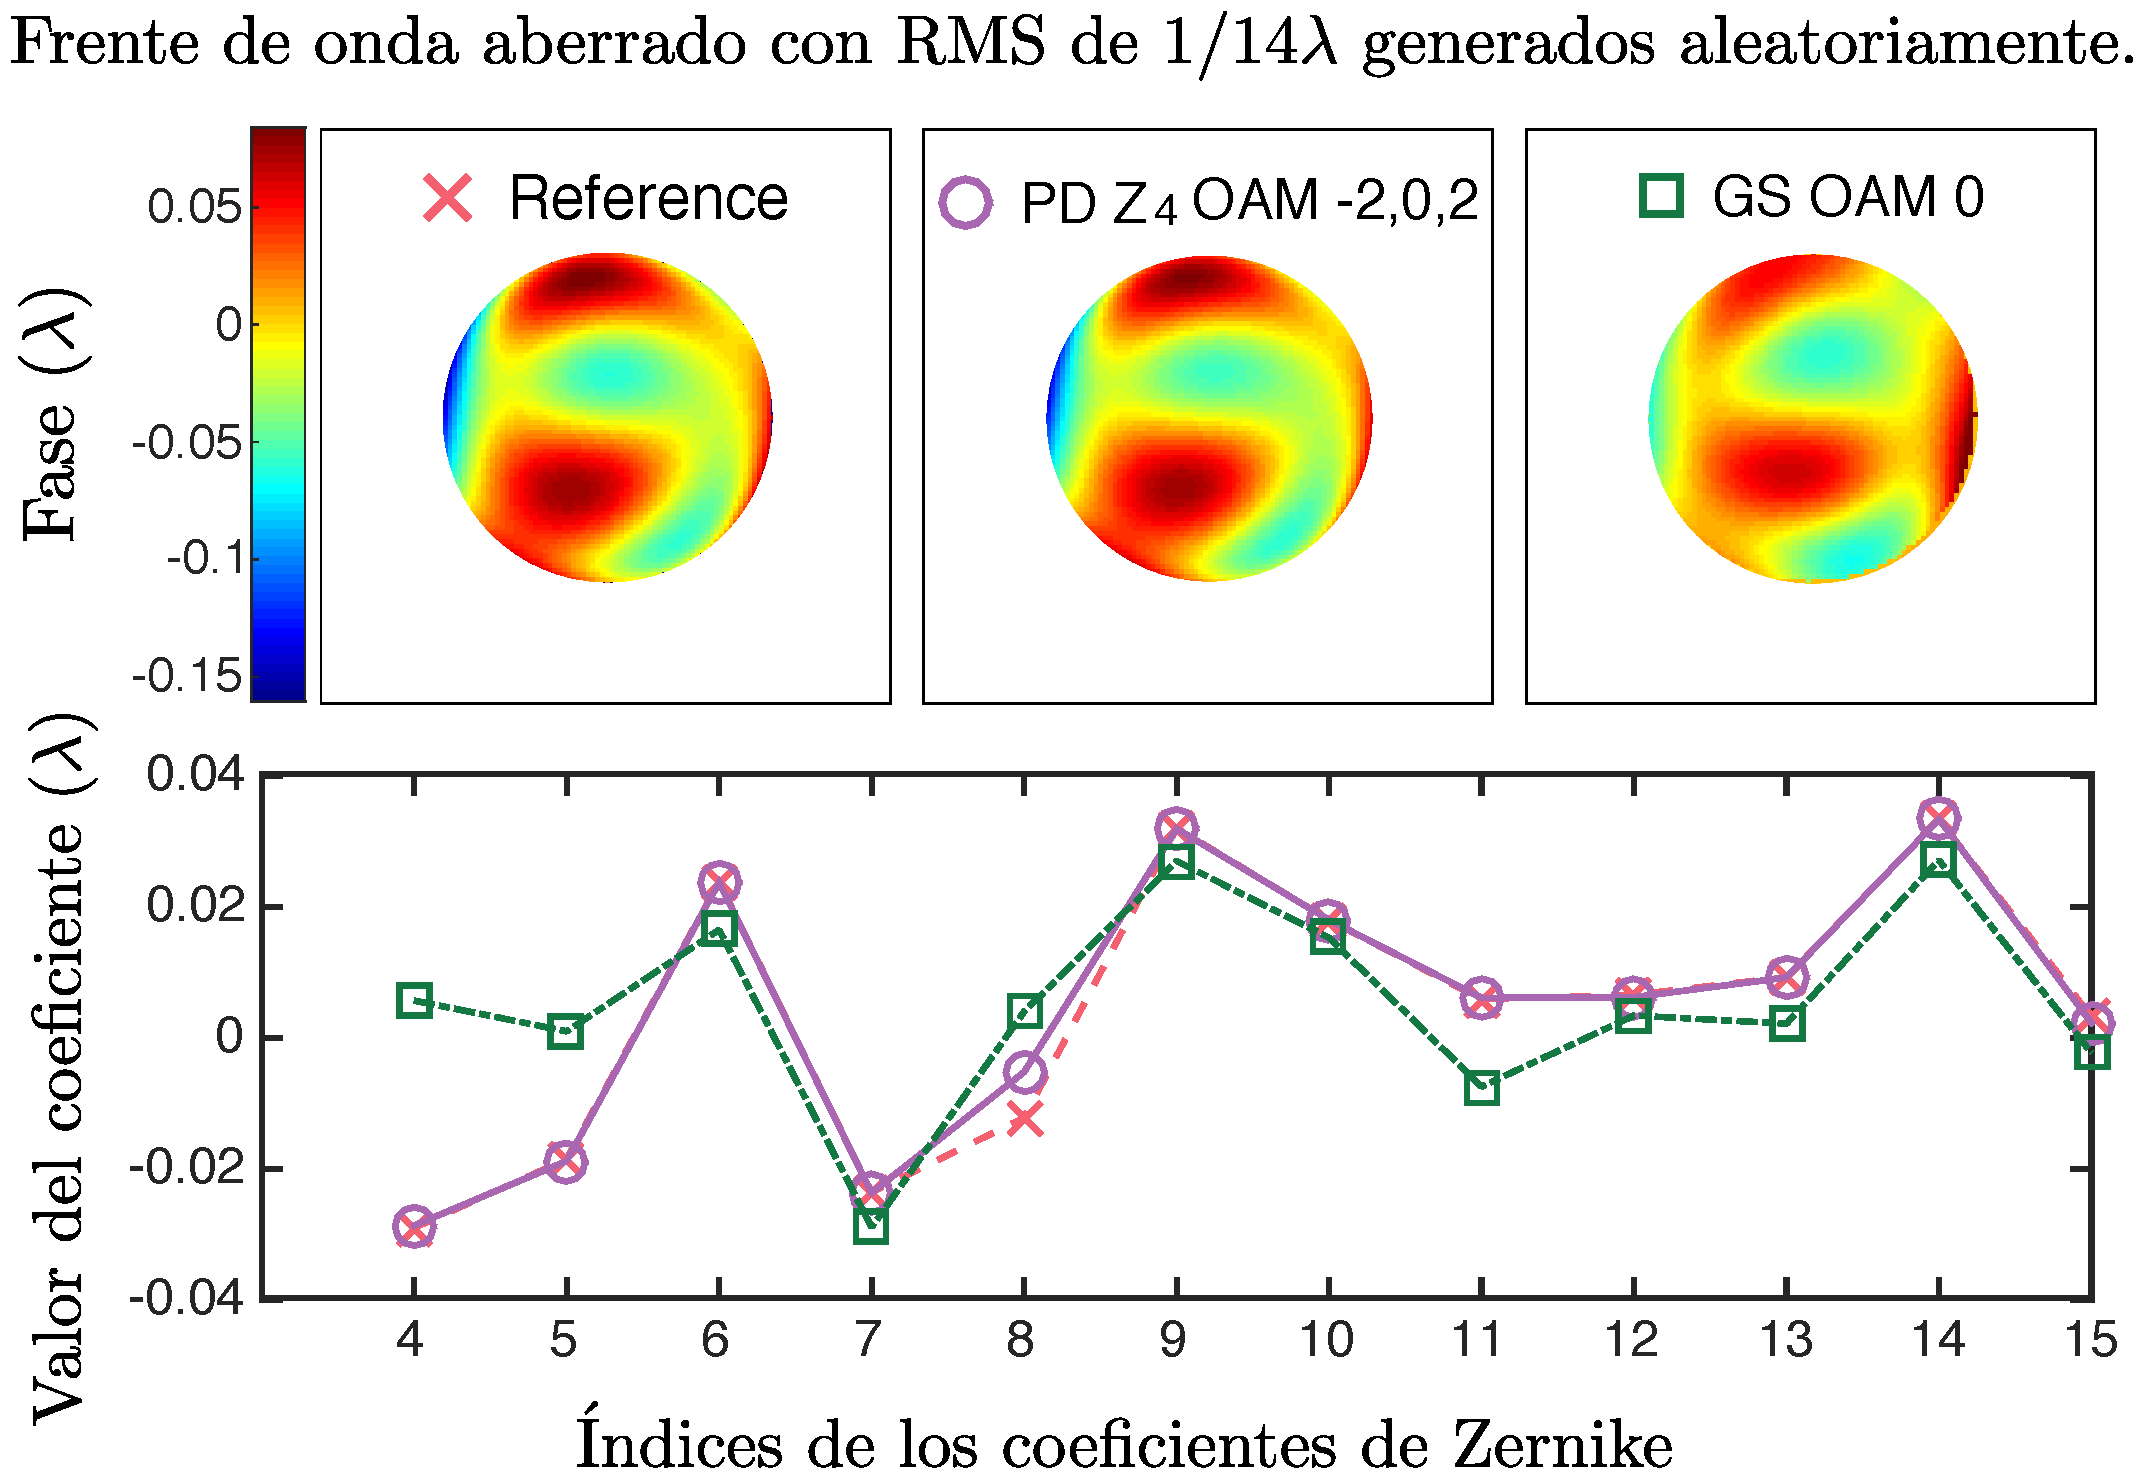
\includegraphics[scale=.3]{phase_comparison_esp.pdf}
\caption[Resultados visuales de simulaciones de PD coherente para
aberración $1/14\lambda$]{Comparación visual y de coeficientes entre uno de los frentes
  de onda aleatorios de escala $1/14\lambda$ y las fases reconstruidas
  con PD y GS.} 
\label{fig:ChPD_visual_comparison}
\end{figure}
Después de un cuidadoso análisis de los resultados, se puedo concluir que hacer un
incremento en la redundancia aumentando la cantidad de imágenes de
entrada tiene un efecto positivo sobre la precisión. Eso se ve
reflejado en la mejor reconstrucción de PD de 9 imagenes con respecto
al de tres, y la mejor reconstrucción de ste último con respecto al GS
de una sola imagen.  Asimismo, identificamos que el desempeño del
método mejora cuando se usan VO con cargas topológicas de orden más
alto, y que la combinación de diversidades espiral de mismo valor pero
signo contrario es preferible a una variedad de cargas de mismo
signo. Creemos que una razón importante por la cual los resultados con
vórtices de $l=2$ son mejores que los de $l=1$ y estos a su vez
mejores que los haces Gaussianos $l=0$ es el hecho de que tienen un
tamaño mayor. Al ocupar una parte mayor de la imagen los cambios en el
perfil debidos a las aberraciones son más evidentes y pueden ser
muestreados con una mayor cantidad de píxeles. Adicionalmente, se
demostrado que las
singularidades de VOs con cargas topológicas mayores a 1 son altamente
inestables y tienden a
dividirse en varios VOs de carga menor ante la presencia de
aberraciones \citepChPD{Dennis2009,Dennis2012}. Por otra parte, pensamos que 
incluir VO con carga negativa y positiva es preferible ya que se le
introducen al método máscaras de diversidad cuya redundancia puede ``desenvolver''
aberraciones simétricas. Una aberración simétrica puede afectar de
distinta forma vórtices ópticos cuya fase se envuelve en sentido
derecho, y vórtices cuya fase se envuelve hacia la izquierda.

\subsubsection{Discusión sobre el método Gerchberg-Saxton}
Analizar correctamente los resultados de la Fig.~\ref{fig:ChPD_RMS_error} depende de entender las diferencias entre la
reconstrucción con GS y la reconstrucción con PD. Comenzaremos por
identificar algunas propiedades de la reconstrucción con el método GS.

El método GS es un algoritmo cíclico de una sola imagen en el cual se
llega a encontrar la fase de un frente de onda haciendo múltiples
propagaciones hacia adelante y hacia atrás del sistema óptico. En este
caso el sistema consiste en la segunda lente de un 4F y las
propagaciones suceden entre el plano de Fourier donde está el SLM y el
plano imagen donde se registran con la CCD. El
algoritmo que implementamos se ilustra de forma gráfica en la
Fig.~\ref{fig:GS_algorithm} y se describe a continuación.
\begin{figure}[h!]
\centering
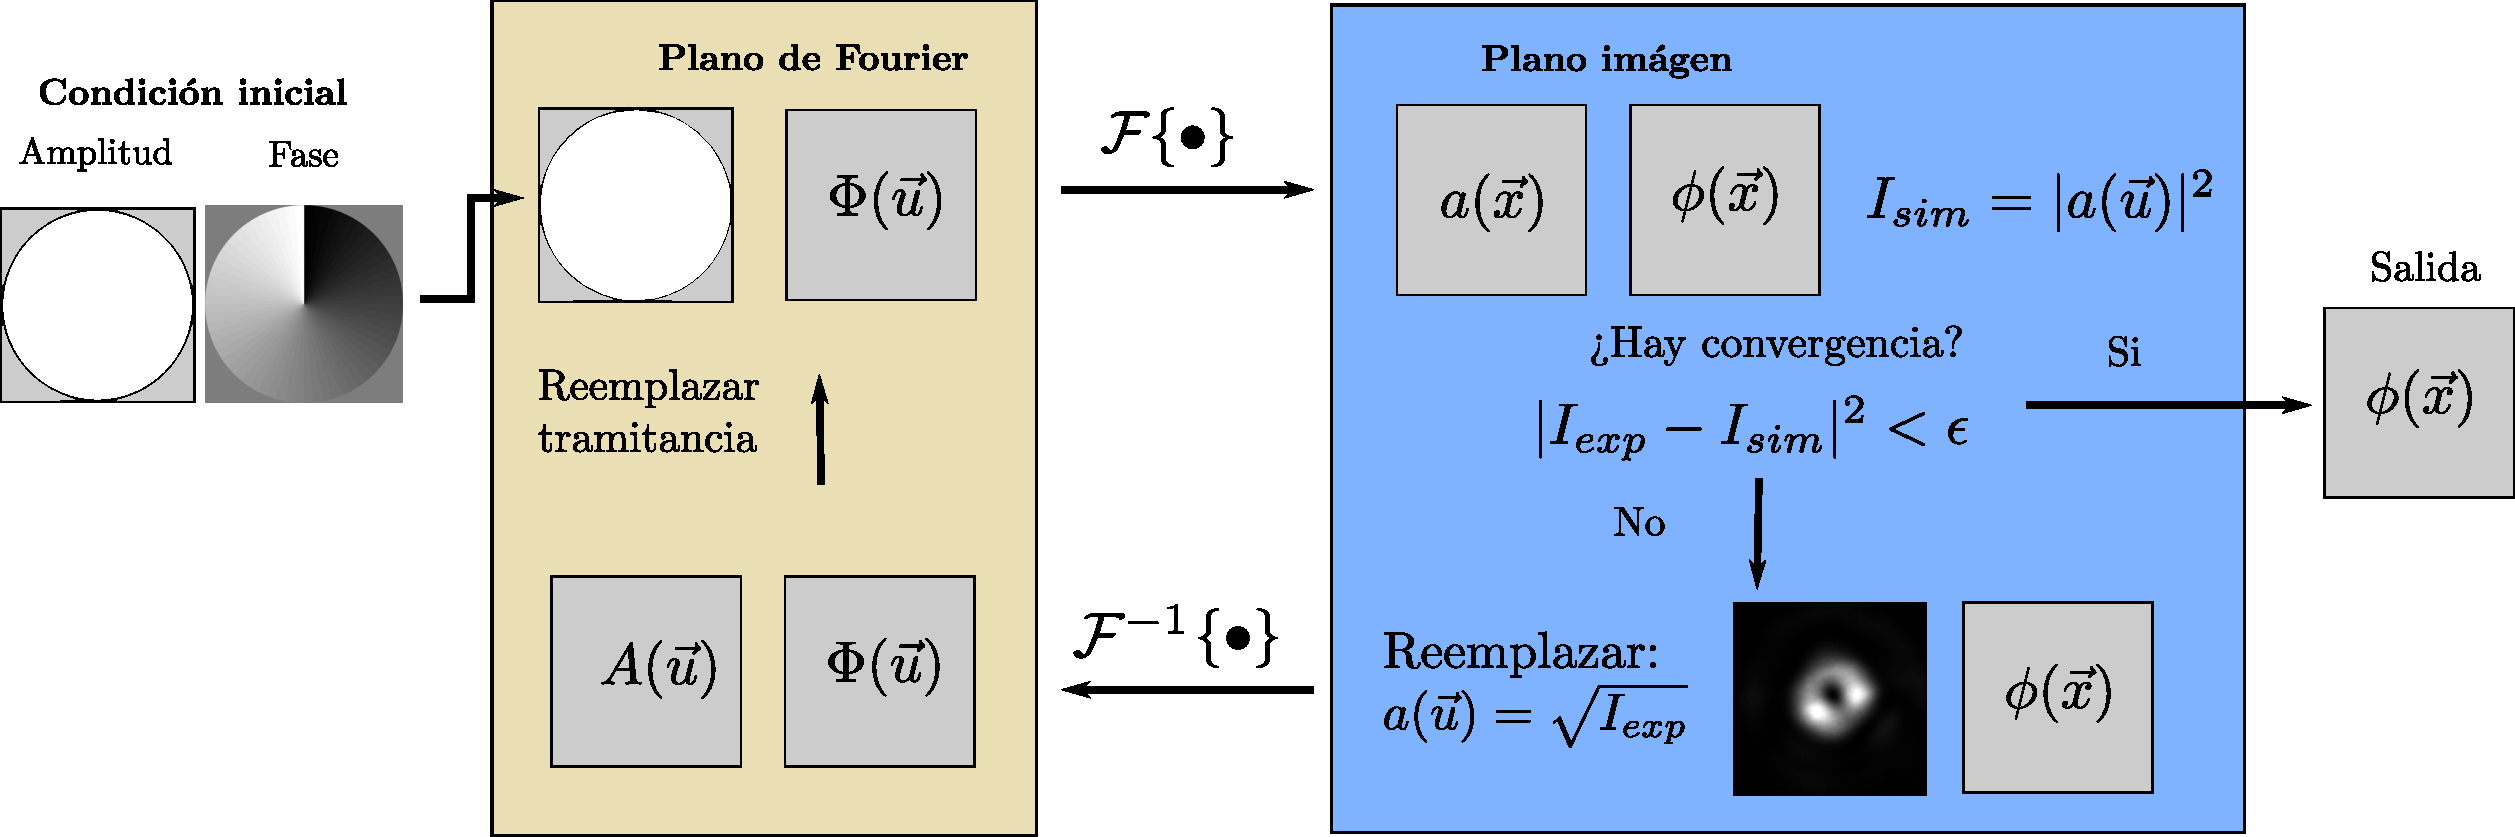
\includegraphics[scale=.36]{GS_algorithm.pdf}
\caption[Algoritmo de GS]{Diagrama de flujo de nuestra implementación
  del método de múltiples propagaciones de Gerchberg-Saxton.} 
\label{fig:GS_algorithm}
\end{figure}
Se parte de un campo complejo conocido en un plano
de Fourier, que se debe propagar por medio de una FT a través del
sistema para obtener el campo en el plano imagen. La amplitud del
campo resultante se reemplaza por la raíz cuadrada de la intensidad
medida experimentalmente, y el resultado se propaga en sentido
contrario a través del sistema por medio de una FT inversa. De nuevo
en el plano de Fourier, la amplitud del campo se reemplaza por una
equivalente a la que habría en la entrada del sistema y se repite el
ciclo hasta que la fase converja a la aberración del sistema que
produce intensidades a la salida iguales a las intensidades tomadas
experimentalemente.  
Si el campo óptico propuesto en el plano de
Fourier del sistema es tal que su imagen resulta similar a la imagen
de entrada, la convergencia es casi segura, el error desciende en cada
iteración y se necesita de muy pocas
iteraciones para alcanzar convergencia. Este es el caso del ejemplo
que mostramos en la Fig.~\ref{fig:ChPD_visual_comparison}. En estos
casos podemos suponer que el algoritmo ha retornado un mínimo
global. Sin embargo, aberraciones de mayor magnitud, o con formas
complejas, pueden hacer que el error aumente antes de comenzar a
descender, y entregar resultados que, aunque generan intensidades
similares a las imágenes experimentales, no 
tienen fases similares a la fase de referencia.  Estos serían entonces
mínimos locales, y no representarían una solución aceptable a la hora
de comparar con una métrica como el RMS del frente de onda. Este
fenómeno ha sido estudiado ya por varios autores
\citepChPD{Paxman1992,Jesacher2007} que han mostrado que la unicidad
de la solución no está garantizada cuando se ejecutan métodos de
propagación como el GS.  
La presencia de mínimos locales y la
imprecision pueden entenderse si se observa 
que, a diferencia de métodos basados en búsqueda del gradiente, en los
cuales la fase se compone de forma parametrizada, el proceso cíclico
del GS retorna la fase como una imagen por el simple hecho de propagar campos complejos
en forma iterativa. Como resultado se corre el riesgo de obtener distribuciones
de fase que no representan adecuadamente el sistema.  Un ejemplo muy bueno de situaciones en las
cuales se presenta ese fenómeno es el que se ilustra en la Fig.
\ref{fig:visual_comparison}. Esta figura muestra el resultado de la
reconstrucción de fase con varios métodos cuando las aberraciones son
grandes (RMS $>1\lambda$) y se puede ver claramente que PD sigue siendo
altamente preciso, y que la solución
con el método de GS (cuadrados rojos) llegó a un mínimo que no
corresponde a la referencia. En este caso se muestra además que la
solución con el método de GS mejorado con VOs devuelve una fase espiral
aberrada que no corresponde a la fase espiral de referencia. Además hemos
visto que en algunos casos las múltiples propagaciones
producen singularidades de fase adicionales no ubicadas en el centro
de la imagen. 
\begin{figure}[h!]
\centering
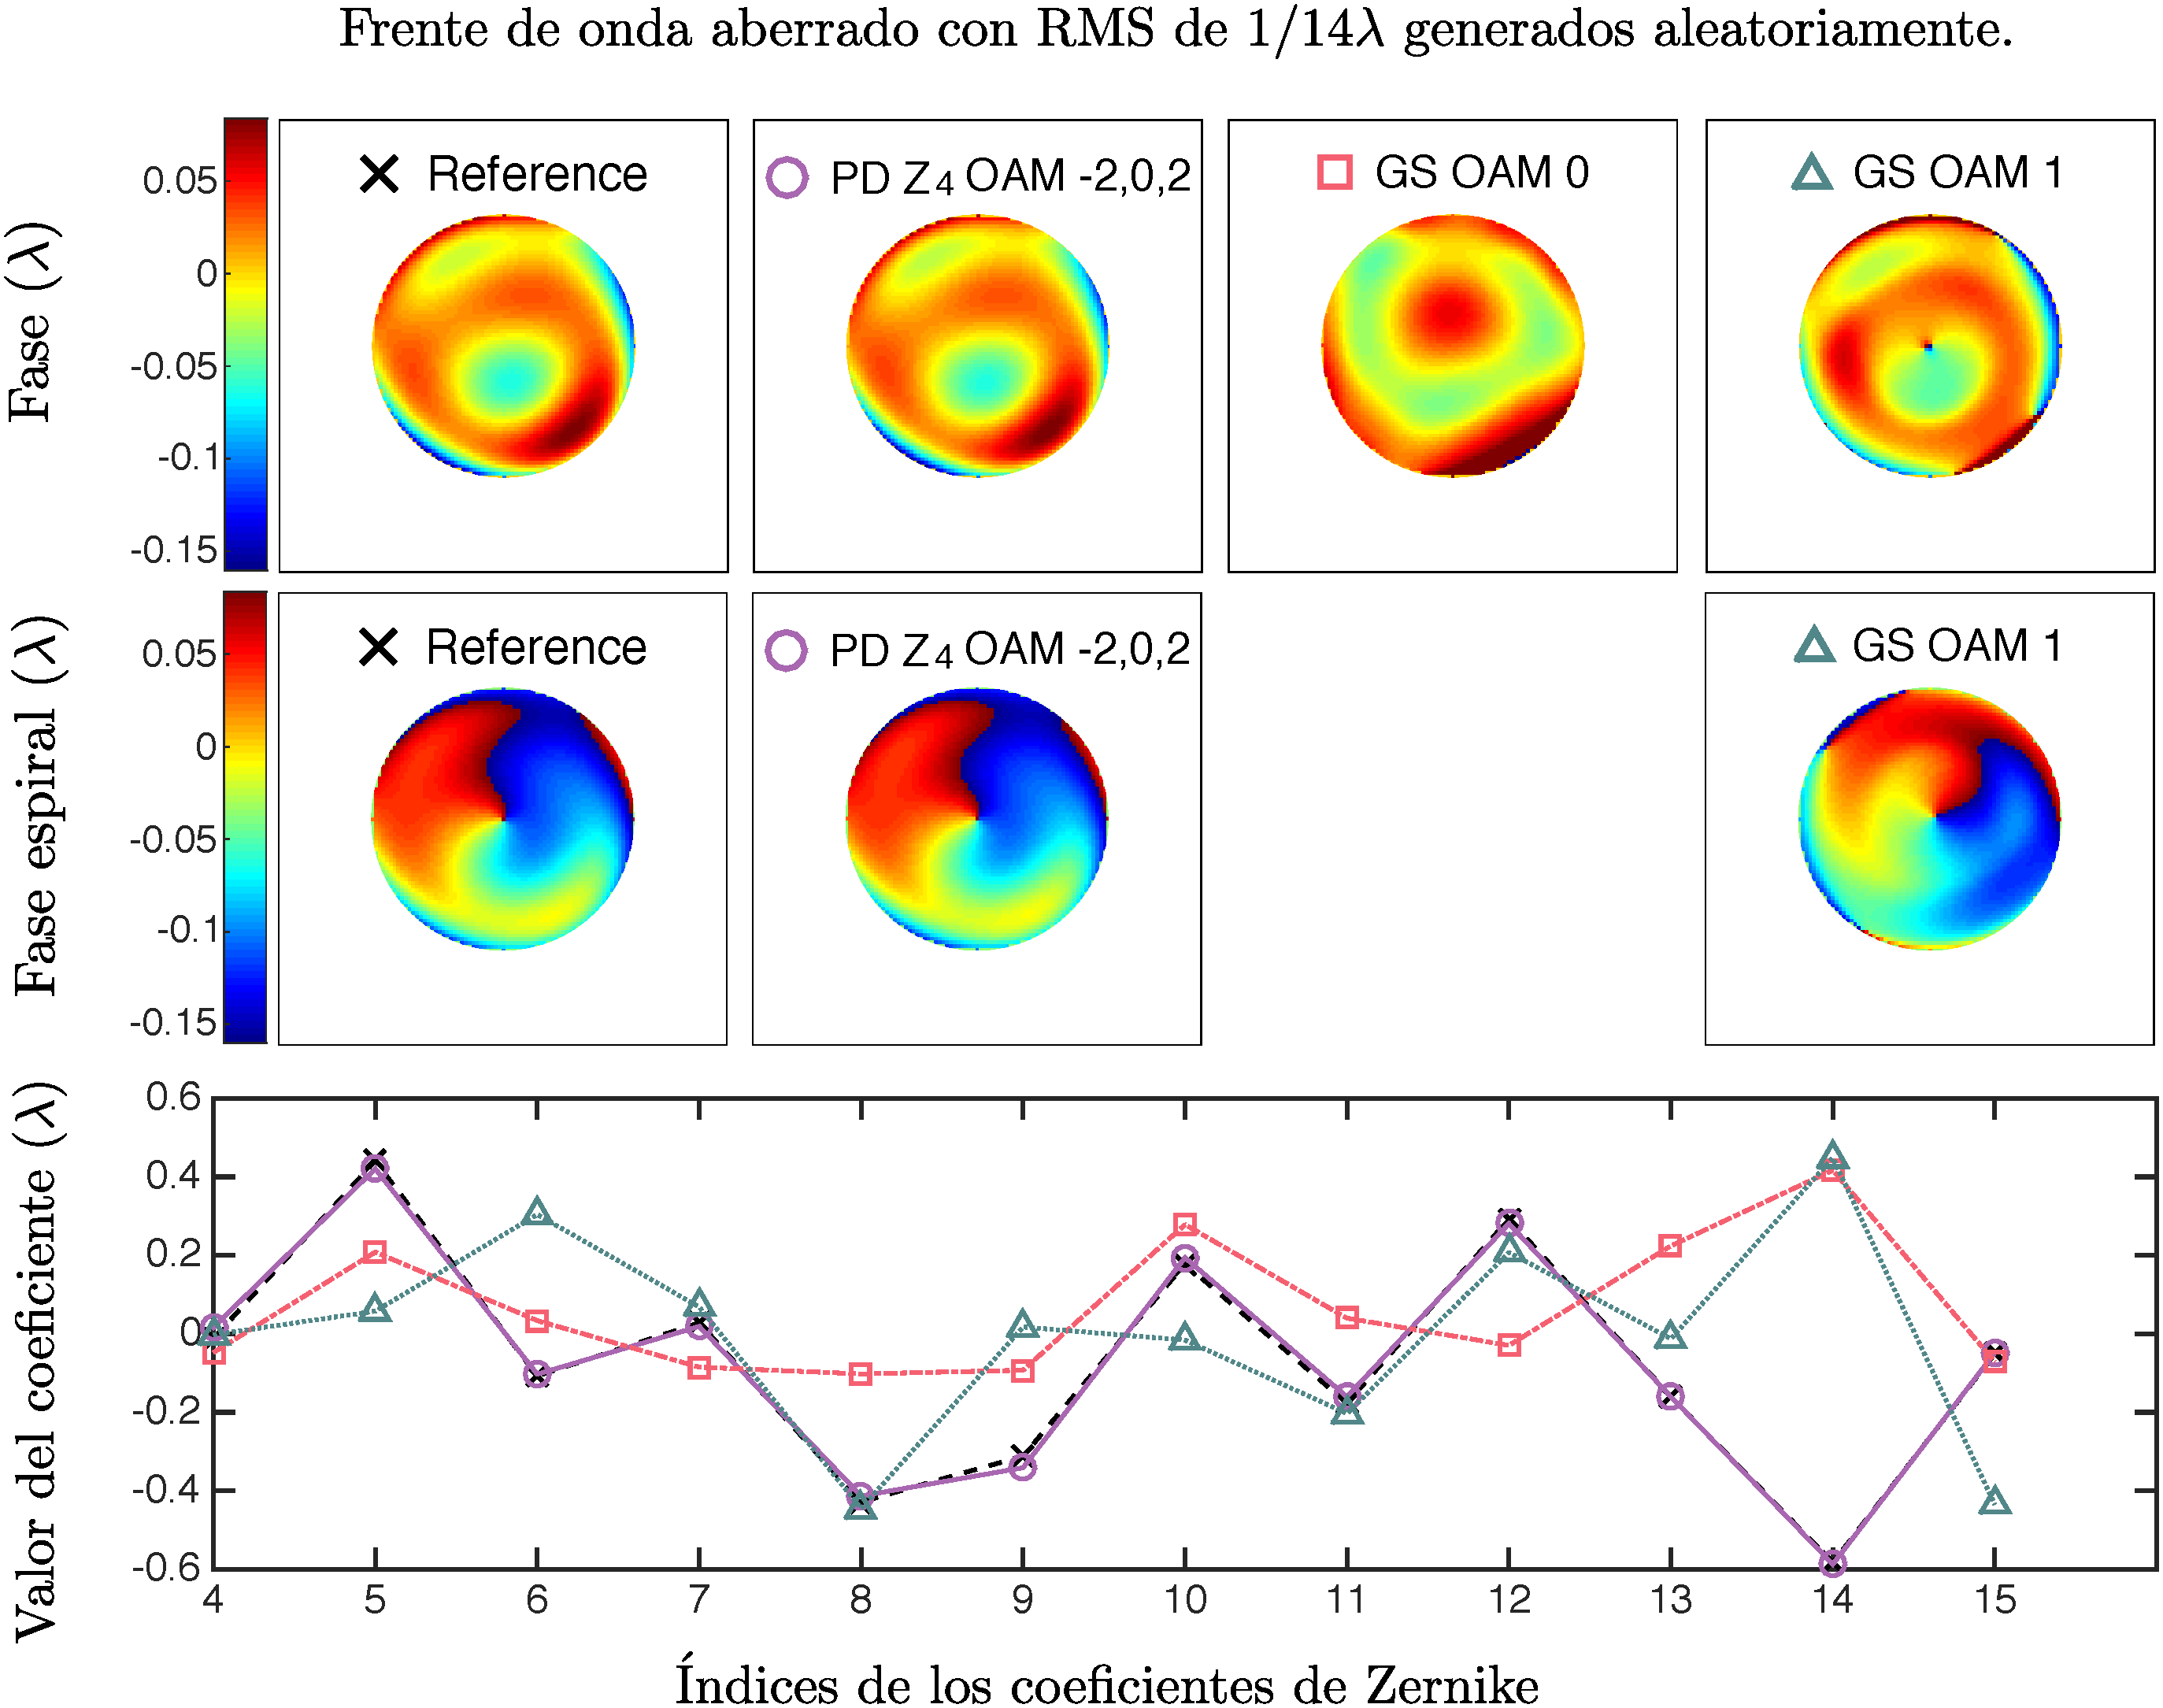
\includegraphics[scale=.3]{phase_comparison_esp_2.pdf}
\caption[Resultados visuales de simulaciones de PD coherente para
aberración $1\lambda$]{Comparación visual y de coeficientes entre uno de los frentes
  de onda aleatorios de escala $1\lambda$ y las fases reconstruidas
  con PD y GS. En este caso se incluye también el resultado del GS con
VOs porque al restar la fase espiral y proyectar a la base de Zernike
se obtuvieron mejores resultados que sin VOs.} 
\label{fig:visual_comparison}
\end{figure}
Más aún, las propagaciones del GS pueden propiciar la aparición de
aberraciones del tipo Pistón ($Z_0$) o plano inclinado
($Z_{1,2}$) que no afectan la forma de la distribución de intensidad
pero si distorsionan la máscara espiral aberrada y que 
pueden invalidar la comparación con la fase de referencia. 
A fin de que la comparación entre el método de GS y el PD sea justa se
sustrajeron las máscaras espiral cuando estaban presentes y la fase
del frente de onda se proyectó al equivalente en la  base Zernike tal
y como muestra en el Capítulo 5 de \citepChPD{Schmidt2010}. Con esto
se pudieron extraer los coeficientes correspondientes a los datos de
cuadros rojos y triángulos azules de la figura
\ref{fig:visual_comparison}. 
En términos generales, se observó que aún cuando el método de GS
encontraba distribuciones de fase que llevaban a intensidades
similares a las intensidades esperadas, estas fases no eran
suficientemente cercanas a la fase de referencia que se esperaba. Esto
se evidencia cuantitativamente en los altos valores del error RMS y su
desviación estandar en las curvas y barras de las
Fig.~\ref{fig:ChPD_RMS_error}(a) y (b).
% Viendo que distribuciones de fase aleatorias probablemente impedirían
% implementar un método de análisis de convergencia basado en búsqueda
% de una variación del error por debajo de un cierto umbral, decidimos
% ejecutar el algoritmo de GS de tal forma que se detuviera una vez
% hubieran pasado 60 iteraciones independientemente del caso. Esto
% aseguraría que las simulaciones que iban en buen camino alcanzaran un
% cambio en el error suficientemente bajo, y le impediría a las
% soluciones que divergían seguir aumentando el error indefinidamente. 


\subsubsection{Sobre las limitantes del método}
La superioridad del método PD viene con la desventaja de implicar un
mayor tiempo de procesamiento. Mientras que las reconstrucciones con
GS pueden tardar alrededor de 30 segundos, la reconstrucción con el PD
de 3 imágenes tarda 6 minutos y la de PD con 9 tarda 22 minutos. Esto
se debe a que el algoritmo es más complejo y las funciones de
minimización que buscan la mayor pendiente necesitan de una mayor cantidad
de evaluaciones de los funcionales de la
Eq.~(\ref{eq:metric_coherent}) y la
Eq.~(\ref{eq:metric_coherent_OAMs}) para poder ensamblar el gradiente 
numéricamente. Todos los resultados fueron obtenidos a partir de
código programado en el lenguaje de programación Matlab$\circledR$ y
no han sido optimizados para mejorar la velocidad de
procesamiento. Futuras implementaciones paralelizadas de los
algoritmos podrían sacar provecho de lenguajes de programación de bajo
nivel como \textbf{C++} y de una \textbf{Unidad de Procesamiento Gráfico} (\acrshort{GPU})
para mejorar los tiempos de reconstrucción y hacer del método una
alternativa viable en aplicaciones donde la velocidad sea importante. 

\subsection{Resultados experimentales}
\label{sec:ChPD_resultados_experimentales}

El método de PD con iluminación coherente mejorado con VOs también fue
probado con aberraciones inducidas en sistemas ópticos reales. A
continuación se describe el montaje óptico, el experimento planteado y
se muestran los resultados. 

\subsubsection{Montaje óptico} 
El montaje experimental usado para la caracterización de aberraciones
se puede observar en la Fig.~\ref{fig:exp_setup}. Como fuente de
iluminación se ha utilizado una fuente laser de 532nm con polarización
vertical y modo $TEM_{0,0}$ que puede observarse en la parte derecha de la imagen. Este
láser de estado sólido produce un haz con polarización ligeramente
elíptica; con el fin de garantizar un estado de polarización lineal
vertical hemos introducido un polarizador (P1) con recubrimiento delgado a
base nanopartículas que tiene una alta relación de
extinción (10.000:1) marca THORLABS referencia LPVISB050. Una vez
seleccionado el estado de polarización, el haz continúa su recorrido 
hasta el extremo izquierdo de la mesa óptica donde cambia de dirección
para luego pasar por un filtro espacial (SF) que se ilustra a la izquierda
de la Fig.~\ref{fig:exp_setup}. El SF permite eliminar
contenidos con altas frecuencias como speckle y obtener un perfil
 bien definido que pueda ser aproximado por una función Gaussiana. La
 lente L1 cuya distancia focal de 10 cm coincide con la distancia hasta
 el pinhole del SF, y colima el haz que diverge a causa del
 objetivo de microscopio de 20x en el SF. 

\begin{figure}[h!]
\centering
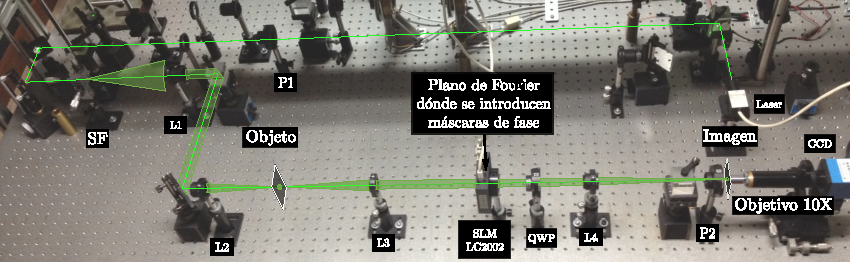
\includegraphics[scale=1]{PD_setup_big.pdf}
\caption[Montaje experimental para reconstrucción de fase con PD]{Montaje experimental para la caracterización de aberraciones
en VO.} 
\label{fig:exp_setup}
\end{figure} 

Una vez colimado, el haz queda de un
 diámetro de aproximadamente 2cm y continúa su recorrido hasta la
 lente L2. La lente L2 de distancia focal 10cm enfoca el haz en un
 plano que en adelante llamaremos plano objeto y que está a una
 distancia de 15cm de L3. Los elementos que se encuentran a partir de este
 punto conforman el sistema formador de imagen a ser
 analizado.
% y en este caso resulta muy similar a un microscopio óptico para
% observar el plano objeto. 
El sistema formador de imagen
 que implementamos es un sistema 4F conformado por las lentes L3 y
 L4. El plano objeto del sistema está a una distancia de L3 que coincide con su
 distancia focal, y asimismo el SLM está a una distancia focal a la
 derecha de L3. Esta configuración asegura que las diversidades de
 fase introducidas al modulador actúen 
 exactamente en el plano donde se encuentra la FT del objeto.       
Por otra parte, la distancia focal de L4 coincide con la distancia
entre el plano del SLM y la lente L4. Esto hace que el haz tenga un
mismo tamaño entre L3 y L4 y que la distribución de intensidades que
se observa en el plano imagen corresponda a una antitransformada del
campo a la salida del SLM. Con esta configuración hemos emulado el
montaje que se ilustró en la figura \ref{fig:set-up} en la sección
anterior. 

Las imágenes que sirven de entrada al algoritmo son capturadas por un
ocular de microscopio marca Newport con aumento de 10x acoplado a una cámara
CCD de resolución 1280x960 marca \textit{Imaging Source} modelo DMK
41BU02.H. Con el fin de capturar con alta precisión las imagenes que corresponden al
primer orden de difracción en el plano imagen, hemos ubicado la cámara
sobre una base con libertad de movimiento en X y Y controlada con
desplazadores micrométricos. El desplazador que actúa en la dirección
perpendicular al haz permite ubicar el ocular ligeramente desplazado
del haz de tal manera que sólo entre la luz correspondiente al primer
orden de difracción. 

\subsubsection{Análisis de resultados}

El montaje en su totalidad tiene aberraciones ópticas que se deben
tanto a la alineación y calidad de los elementos ópticos como a la
capacidad de modulación del TN-SLM. Esas aberraciones son las
responsables de que los VOs sin corrección presentados en el capítulo
anterior tengan una mala calidad. En esta sección mostraremos uno de
los resultados obtenidos con el montaje descrito anteriormente. Con el
fin de evaluar la capacidad del método para recuperar aberraciones
conocidas y no solo las aberraciones inherentes al sistema hemos
añadido una aberración tipo trébol de magnitud $1\lambda$ a todas las
imágenes. Las aberraciones tipo trébol corresponden al
polinomio 10 de la base de Zernike y su perfil de fase se puede
observar en la Fig.~\ref{fig:trefoil_aber}.  

\begin{figure}[h!]
\centering
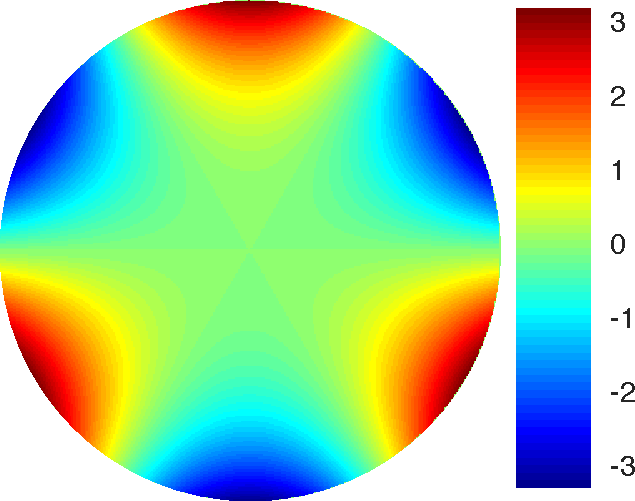
\includegraphics[scale=.4]{trefoil.pdf}
\caption[Aberración tipo trébol.]{Mapa de fase de una aberración tipo
  trébol de valor $1\lambda$.} 
\label{fig:trefoil_aber}
\end{figure} 

La introducción de una aberración conocida se hace por medio del mismo
SLM sumando la máscara de la aberración tipo trébol a las máscaras 
originales usadas en la simulación. %\ref{fig:mixed_mask}. 
Esta aberración no solo nos permite probar el
método en una condición extrema, sino que también permite evaluar
su capacidad para encontrar aberraciones conocidas. 
La Fig.~\ref{fig:exp_results}(a) muestra tres grupos de imagenes, en
la primera fila de cada grupo, se resaltan dentro
de un rectángulo verde 3 de las 9 imágenes de entrada ($d_j^l$)
adquiridas cuando la diversidad espiral es $l=0,1,2$, las diversidades
de aberración son $j = 0\lambda, 0.5\lambda$, y  $-0.5\lambda$ de
astigmatismo, y se ha sumado a todas la aberración tipo trébol.   
\begin{figure}[h!]
\centering
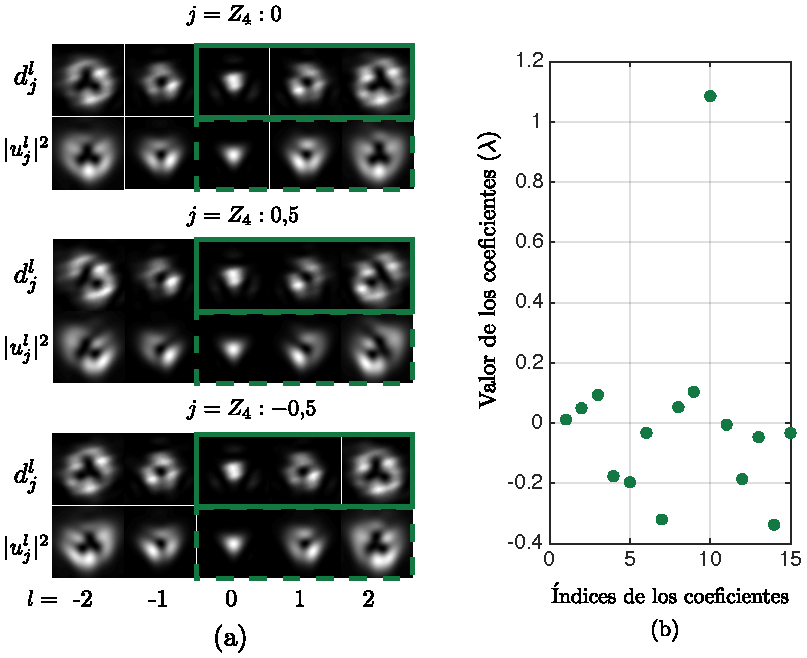
\includegraphics[scale=1]{experimental_results_07032015_small.pdf}
\caption[Resultados experimentales de la reconstrucción de fase con
PD.]{(a) Imagenes experimentales de
  entrada $d_j^l$ vs imágenes simuladas $|u_j^l|^2$ cuando el PD ha
  alcanzado convergencia y se han encontrado las aberraciones del
  sistema $\phi$.  (b) Coeficientes de Zernike que componen $\phi$.} 
\label{fig:exp_results}
\end{figure} 

Las nueve imagenes dentro de recuadros con línea sólida son la
entrada al algoritmo de PD y las imágenes en recuadros con líneas
discontinuas corresponden a las imagens sintéticas ($|u_j^l|^2$) obtenidas
cuando el método de búsqueda del gradiente ha alcanzado su punto de 
convergencia. Se puede observar que las imagenes
recuperadas por nuestro método no sólo emulan con alta precisión las
imagenes usadas como entrada ($l=0,1,2$) sino, también otras imagenes que no
fueron incluidas. En este caso las no incluidas corresponden a
diversidades de fase espiral $l=-2,-1$. El hecho de que logremos emular el comportamiento
del montaje experimental en casos que no fueron usados por el método
es un buen indicador de que se obtuvo una solución global, y que la
aberración del sistema es precisamente la recuperada. Luego, la
Fig.~\ref{fig:exp_results}(b) muestra los valores de los 15
coeficientes de 
Zernike que componen la aberración recuperada y lo primero que se puede
observar es un pico con valor de  $1.08\lambda$ en el coeficiente
número 10, muy distinto a las otras componentes de magnitudes menores
a $0.4\lambda$, que comprueba la exactitud de la solución.   

Finalmente, la Fig.~\ref{fig:exp_correction} muestra VOs de calidad mejorada obtenidos
luego de compensar el frente de onda recuperado al frente de
onda nominal $j = Z_4:0$.  

\begin{figure}[h!]
\centering
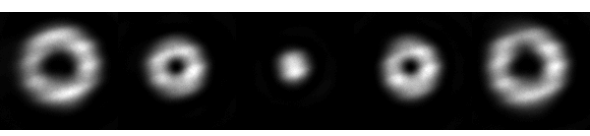
\includegraphics[scale=1.5]{PSF_comparison_experimental_results_07032015.pdf}
\caption[VO registrados luego restar las aberraciones detectadas
  con PD.]{Imagenes de VO tomadas luego de restar las aberraciones
    reconstruidas con PD.}  
\label{fig:exp_correction}
\end{figure}

Este resultado demuestra que se logró implementar un sistema capaz de
generar, caracterizar y corregir VO mediante el uso de un SLM. 

Fuera de eso, y dado que los VO tienen gran sensibilidad ante ciertas
aberraciones, el método desarrollado puede ser utilizado como una
herramienta de metrología óptica para la caracterización de sistemas
formadores de imagen. 

En el marco del proyecto de grado se generó una
publicación científica que ha sido enviada a la revista Optics Letters
y está en proceso de revisión. En esta publicación se propone nuestra implementación
como una posible alternativa paran la caracterización de sistemas
formadores de imagen que puedan ser iluminados con fuentes
coherentes. 

\newpage
\pagebreak[4]
\bibliographystyleChPD{SETUP/ezspanish}
\bibliographyChPD{References/Ch_PD}

